\chapter {Implicit solution methods for coupled fields} \label{chapter:implicit_meth}

This chapter presents the most common strongly coupled/implicit methods employed to solve coupled field problems.
This presentation seeks to provide a literature overview of the available approaches.

% More thorough description of the chapter
% Two main ways of realizing a strongly coupled approach to the solution of the coupled problem are presented.
% The first focuses on fixed-point solvers and acceleration/stabilization techniques for them.
% The second deals with approaches based on the Newton-Raphson method, with the main problem tackled being an efficient and accurate approximation to the Jacobian.\jvc{In the end, rewrite the description of the chapter}

\section{Equations to be solved}

For the sake of clarity, the discretized equations of the thermo-mechanical problem at the next time instant, \(n+1\)e are recovered here
\begin{gather}
    \mathbf M \ddot{\mathbf u}_{n+1} +\mathbf f_u^\text{\;int}(\bm \uptheta_{n+1}, \mathbf u_{n+1})-\mathbf f^\text{\;ext}_{u,n+1}=\mathbf 0, \label{eq:mech_problem} \\
    \mathbf C \dot{\bm \uptheta}_{n+1} + \mathbf K \bm \uptheta_{n+1} +\mathbf f_\theta^\text{\;int}(\bm \uptheta_{n+1}, \mathbf u_{n+1})-\mathbf f^\text{\;ext}_{\theta,n+1}=\mathbf 0. \label{eq:therm_problem}
\end{gather}
The complete definition of the material incremental discretized thermo-mechanical initial boundary value problem can be found in Chapter~\ref{ch:thermo_mechanical_problem}.

As only partitioned approaches are considered, the thermal and mechanical problems are solved separately, i.e., Equation~\eqref{eq:mech_problem} is solved considering a fixed temperature, and Equation~\eqref{eq:therm_problem} is solved assuming a fixed configuration.
To ease the discussion, consider the existence of two functions \(\pazocal U_{n+1}\) and \(\pazocal T_{n+1}\) that represent these solution procedures at timestep \(n+1\).
These so-called mechanical and thermal solvers satisfy
\begin{highlight}[innertopmargin=-5pt]
\begin{gather}
  \pazocal U\colon \mathscr K_{\theta, n+1}\to \mathscr K_{u,n+1},\quad \mathbf u = \pazocal U_{n+1}(\bm \uptheta),\\
  \pazocal T\colon \mathscr K_{u,n+1}\to \mathscr K_{\theta, n+1},\quad \bm \uptheta = \pazocal T_{n+1}(\mathbf u).
\end{gather}
\end{highlight}
See Chapter~\ref{ch:thermo_mechanical_problem} for detailed information on them.
In the following, the subscripts on the solvers will be dropped to avoid clutter.

The goal now is to consider functions, built from \(\pazocal U\) and \(\pazocal T\), whose roots are also the solutions to the thermo-mechanical problem (Equations~\eqref{eq:mech_problem} and \eqref{eq:therm_problem}).
Several examples can be provided.
The most appropriate for the current use case are presented in what follows.
They can be found in \cite{uekermann_partitioned_2016} in the context of fluid-structure interaction (FSI).

Consider the residues defined as,
\begin{highlight}
\begin{equation} \label{eq:def_res_jacobi}
  \pazocal R_\text{J}\colon \mathscr K_{u,n+1}\times\mathscr K_{\theta,n+1} \to K_{u,n+1}\times\mathscr K_{\theta,n+1},\quad  \pazocal R_\text{J}(\mathbf u, \bm \uptheta) =
  \left\{\begin{array}{c}
  \mathbf u - \pazocal U(\bm \theta)\\
  \bm \uptheta - \pazocal T(\mathbf u)
  \end{array}\right\},
\end{equation}
\end{highlight}
and
\begin{highlight}
\begin{equation} \label{eq:def_res_gauss_seidel}
  \pazocal R_\text{GS}\colon \mathscr K_{\theta,n+1} \to\mathscr K_{\theta,n+1},\quad \pazocal R_\text{GS}(\bm \uptheta) =
  \bm \uptheta - \pazocal T\circ \pazocal U(\bm \uptheta),
\end{equation}
\end{highlight}
or
\begin{equation}
  \pazocal R^*_\text{GS}\colon \mathscr K_{u,n+1} \to\mathscr K_{u,n+1},\quad \pazocal R^*_\text{GS}(\mathbf u) =
  \mathbf u - \pazocal U\circ \pazocal T(\mathbf u),
\end{equation}
where the subscript "J" stands for Jacobi and the subscript "GS" for Gauss-Seidel.
The reason for this choice of subscripts is made clear in Section~\ref{sec:fixed_point_approach}.

Since the methods described below for the solution of nonlinear systems of equations apply to both functions \(\pazocal R_\mathrm{J}\) and \(\pazocal R_\mathrm{GS}\), a general function denoted as \(\pazocal R\), whose variable is \(\mathbf x\), is considered instead.
As already stated, the solution for the thermo-mechanical problem (Equations~\eqref{eq:mech_problem} and \eqref{eq:therm_problem}) can be abstracted as the solution of
\begin{equation} \label{eq:abstract_residue_equation}
  \pazocal R(\mathbf x) = 0.
\end{equation}
To obtain simpler expressions in what follows, consider also the function
\begin{equation}
\pazocal S(\mathbf x) = \mathbf x - \pazocal R(\mathbf x),
\end{equation}
whose fixed point is the solution to the nonlinear system of equation in Equation~\eqref{eq:abstract_residue_equation}.

\section{A classification scheme for iterative methods}

Most methods available for the solution of systems of nonlinear equations, such as the one in Equation~\eqref{eq:abstract_residue_equation}, are iterative methods.
They can be more precisely defined lettting \(\mathbf x^{k},\mathbf x^{k-1}, \ldots\), whose superscripts correspond to the loop of the iteration method, be approximants to \(\mathbf x_{n+1}\), whose subscript concerns the timestep

To better understand the landscape of available methods to solve nonlinear systems of equations, the iteration functions are classified according to the information they require following the classification scheme by \cite{traub_iterative_1982}.
Let \(\mathbf x^{k+1}\) be determined uniquely by information obtained at \(\mathbf x^{k}, \mathbf x^{k-1}, \ldots\), including the derivatives of any order of \(\pazocal R\).
Let the function that maps \(\mathbf x^{k}, \mathbf x^{k-1}, \ldots\) into \(\mathbf x^{k+1}\) be called \(\phi\).
Thus
\begin{highlight}
\begin{equation}
  \mathbf x^{k+1}=\phi\left(\mathbf x^{k},\pazocal R(\mathbf x^{k}), J_\pazocal{R}(\mathbf x^k), \dots\right),
\end{equation}
\end{highlight}
where \(\phi\) is called an iteration function, and \(J_\pazocal{R}\) is the Jacobian of \(\pazocal R\).
To prevent clutering \(\mathbf x^k\) will stand for its value as well as for the values of \(\pazocal R(\mathbf x^k)\), \(J_\pazocal{R}(\mathbf x^k)\) and further derivatives of higher order.
Then \(\phi\) is called a \textit{one-point iteration function}.
Most iteration functions that have been used for root-finding are one-point iteration functions. The most commonly known examples are the fixed point schemes and Newton's iteration method.

Next, let \(\mathbf x^{k+1}\) be determined by new information at \(\mathbf x^{k}\) and reused information at \(\mathbf x^{k-1}, \ldots\)
Thus
\begin{highlight}
  \begin{equation}\label{eq:one_point_iteration_function_with_memory}
    \mathbf x^{k+1}=\phi\left(\mathbf x^{k} ; \mathbf x^{k-1}, \ldots\right) .
  \end{equation}
\end{highlight}
Then \(\phi\) is called a \textit{one-point iteration function with memory}.
The semicolon in Equation~\eqref{eq:one_point_iteration_function_with_memory} separates the point at which new data are used from the points at which old data are reused.
The secant iteration function is the best-known example of a one-point iteration function with memory.

Let \(\mathbf x^{k+1}\) be determined by new information at \(\mathbf x^{k}, \omega_{1}\left(\mathbf x^{k}\right), \ldots\), \(\omega_{i}\left(\mathbf x^{k}\right)\), \(i \geq 1\), where \(\omega_i\) denote operations on \(\mathbf x^k\).
No old information is reused.
Thus
\begin{highlight}
  \begin{equation}
    \mathbf x^{k+1}=\phi\left[\mathbf x^{k}, \omega_{1}\left(\mathbf x^{k}\right), \ldots, \omega_{i}\left(\mathbf x^{k}\right)\right].
  \end{equation}
\end{highlight}
Then \(\phi\) is called a \textit{multipoint iterative function}.
Such methods include the Aitken-Steffson method.

Finally, let \(\mathbf z_{j}\) represent the quantities \(\mathbf x^{j}, \omega_{1}\left(\mathbf x^{j}\right), \ldots, \omega_{i}\left(\mathbf x^{j}\right)\), \(i \geq 1\).
Let
\begin{highlight}
  \begin{equation} \label{eq:multipoint_iterative_function_with_memory}
  \mathbf x^{k+1}=\phi\left(\mathbf z^{k} ; \mathbf z^{k-1}, \dots \right) .
  \end{equation}
\end{highlight}
Then \(\phi\) is called a \textit{multipoint iterative function with memory}.
The semicolon in Equation~\eqref{eq:multipoint_iterative_function_with_memory} separates the points at which new data are used from the points at which old data are reused.

In the present work, the criteria used for the choice of the iterative method used fit roughly into the ones provided by \cite{fang_two_2009} for problems in the context the electronic structure problems.
They are
\begin{enumerate}
  \item The dimensionality of the problem is large.
  \item \(\pazocal R(\mathbf x)\) is continuously differentiable, but the analytic form of its derivative is not readily available, or it is costly to compute.
  \item The cost of evaluating \(\pazocal R(\mathbf x)\) is computationally high.
  \item The problem is noisy. In other words, the evaluated function values of \(\pazocal R(\mathbf x)\) usually contain errors.
\end{enumerate}
Thus, the methods chosen must minimize the number of calls to \(\pazocal R\), as it is expensive to compute.
The amount of information saved from previous iterations must also be judiciously chosen as the problem's dimensionality is large, leading to memory limitations.
Finally, the analytical form of the derivative \(\pazocal{R}\) is also not available.
Thus methods that use it must be discarded.

\subsection{Predictor} \label{sec:predictor}

Iterative procedures are considered to solve the thermo-mechanical problem at a given timestep \(n+1\).
As the first value approximating \(\mathbf x_{n+1}\), one can employ the converged value of the previous timestep, \(\mathbf x_n\).
However, a very efficient way to increase the chances of stability and reduce computation time is to predict the optimal initial values at the beginning of every time step \citep{erbts_accelerated_2012, erbts_partitioned_2015, wendt_partitioned_2015}.
The prediction of the new solution by polynomial extrapolation is based on the converged solution of the last two or three timesteps.
This method is based on polynomial vector extrapolation, which is relatively easy to implement, and the extra computational input is negligible.

The maximum polynomial under consideration is of the order two, i.e., the new solution is extrapolated from the results from the last three time steps.
The predictors $\mathbf{x}^{*}$ for the order $p=1$ and $p=2$ polynomials read:
\begin{highlight}[innertopmargin=-5pt]
\begin{gather}
p=1:\quad \mathbf{x}_{n+1}^{*}=2 \mathbf{x}_{n}-\mathbf{x}_{n-1}, \\
p=2:\quad \mathbf{x}_{n+1}^{*}=3 \mathbf{x}_{n}-3 \mathbf{x}_{n-1}+\mathbf{x}_{n-2}.
\end{gather}
\end{highlight}

\subsection{Global Approaches}

Following \cite{dennis_numerical_1996}, the terms "global," as in "global method" or "globally convergent algorithm," are here used to denote a method that is designed to converge to a local minimizer of a nonlinear functional or some solution of a system of nonlinear equations, from almost any starting point.
The methods presented in this chapter do not qualify as global methods since if the initial trial is not close enough to the solution, they will not converge.
There are, however, approaches to mitigate this problem.
The ideas presented below apply with particular relevance to the Newton method (see Section~\ref{sec:newtons_method}) and related procedures.
Their exposition follows \cite{dennis_numerical_1996} where more details can be found.

Consider that the iterative solution method determines \(\Delta \mathbf x^k\) in
\begin{equation} \label{eq:general_update_equation}
  \mathbf x^{k+1} = \mathbf x^k + \Delta \mathbf x^k.
\end{equation}
The two global approaches here considered both come into action after \(\Delta \mathbf x^k\) has been computed by some appropriate method (see from Section~\ref{sec:one_point_iteration_function} on).
At this point, one decides whether to accept the step \(\Delta \mathbf x^k\) or to choose \(\mathbf x^{k+1}\) by a global strategy.

A solution to the system of equations~\eqref{eq:abstract_residue_equation} clearly also satisfies
\begin{equation} \label{eq:minimization_equiv}
  r(\mathbf x) = 0,\quad\text{where }r \equiv \frac{1}{2} \|\pazocal R\|^2_2\colon \mathbb R^n\to \mathbb R,
\end{equation}
so the problem can be regarded as an unconstrained minimization problem, with caveat that local minimizers of \(r\) may not be the solution to the system of equations~\eqref{eq:abstract_residue_equation}.

The basic idea of a global method for unconstrained minimization is geometrically obvious: take steps that lead "downhill" for the function \(r\).
More precisely, one chooses a direction \(\mathbf p\) from the current point \(\mathbf x^{k}\) in which \(r\) decreases initially, and a new point \(\mathbf x^{k+1}\) in this direction from \(\mathbf x^k\) such that \(r(\mathbf x^{k-1})<r(\mathbf x^k)\).
Such a direction is called a descent direction.

An important question to ask is, "What is a descent direction for problem \eqref{eq:minimization_equiv}?".
It is any direction \(\mathbf p\) for which \(\nabla r(\mathbf x^k)^{T} \mathbf p<0\), where
\begin{equation}
  \nabla r\left(\mathbf x^k\right)=J_\pazocal R\left(\mathbf x^k\right)^{T} \pazocal R\left(\mathbf x^k\right),
\end{equation}
where \(J_\pazocal R(\mathbf x^k)\) is the Jacobian matrix of \(\pazocal R\) at \(\mathbf x^k\).
Therefore, the steepest-descent direction for \eqref{eq:minimization_equiv} is along \(-J_\pazocal R(\mathbf x^{k})^{T} \pazocal R(\mathbf x^k)\).

The Newton step for the update equation \eqref{eq:general_update_equation} is (see Section~\ref{sec:newtons_method})
\begin{equation}
\Delta \mathbf x^k_N =  - J_ \pazocal R\left(\mathbf x^k\right)^{-1} \pazocal R\left(\mathbf x^k\right),
\end{equation}
and it is a descent direction, since
\begin{equation}
  \nabla r\left(\mathbf x^k\right)^{T} \Delta \mathbf x^k_N=-\pazocal R\left(\mathbf x^k\right)^{T} J_\pazocal R\left(\mathbf x^k\right) J_\pazocal R\left(\mathbf x^k\right)^{-1} \pazocal R\left(\mathbf x^k\right)=-\pazocal R\left(\mathbf x^k\right)^{T} \pazocal R\left(\mathbf x^k\right)<0
\end{equation}
as long as \(\pazocal R\left(\mathbf x^k\right) \neq \mathbf 0\).
Hence, the appropriateness of these methods to the Newton method and related methods.

Since the Newton step yields a root of
\begin{equation}
  M^k\left(\mathbf x^k+\Delta \mathbf x^k\right)=\pazocal R\left(\mathbf x^k\right)+J_\pazocal R\left(\mathbf x^k\right) \Delta \mathbf x^k,
\end{equation}
it also goes to a minimum of the quadratic function
\begin{equation}
  \begin{aligned}
    \hat{m}^k\left(\mathbf x^k+\Delta \mathbf x^k\right) & \equiv \frac{1}{2} M^k\left(\mathbf x^k+ \Delta \mathbf x^k\right)^{T} M^k\left(\mathbf x^k+\Delta \mathbf x^k\right) \\
    &= \frac{1}{2} \pazocal R\left(\mathbf x^k\right)^{T} \pazocal R\left(\mathbf x^k\right)+\left(J_\pazocal R\left(\mathbf x^k\right)^{T} \pazocal R\left(\mathbf x^k\right)\right)^{T} \Delta \mathbf x^k\\
    & \qquad\qquad\qquad\qquad\qquad+\frac{1}{2} \Delta {\mathbf x^k}^{T}\left(J_\pazocal R\left(\mathbf x^k\right)^{T} J_\pazocal R\left(\mathbf x^k\right)\right) \Delta \mathbf x^k,
  \end{aligned}
\end{equation}
because \(\hat{m}^k\left(\mathbf x^k+\Delta \mathbf x^k\right) \geq 0\) for all \(\Delta \mathbf x^k\) and \(\hat{m}^k\left(\mathbf x^k+\Delta \mathbf x^k_N\right)=0\).
Therefore, \(\Delta \mathbf x^k_N\) is a descent direction for \(\hat{m}^k\), and since the gradients at \(\mathbf x^k\) of \(\hat{m}^k\) and \(r\) are the same, it is also a descent direction for \(r\).

The above development motivates how the global methods to be described are applied, i.e., they are applied to the quadratic model \(\hat{m}^k(\mathbf x)\).
Since \(\nabla^{2} \hat{m}^k(\mathbf x^k)=J_\pazocal R(\mathbf x^k)^{T} J_\pazocal R(\mathbf x^k)\), this model is positive definite as long as \(J_\pazocal R(\mathbf x^k)\) is nonsingular, which is consistent with the fact that \(\mathbf x^k + \Delta \mathbf x^k_N\) is the unique root of \(M^k(\mathbf x)\) and thus the unique minimizer of \(\hat{m}^k(\mathbf x)\) in this case.
Thus, the model \(\hat{m}^k(\mathbf x)\) has the attractive properties that its minimizer is the Newton point for the original problem, and that all its descent directions are descent directions for \(r(\mathbf x)\) because \(\nabla \hat{m}^k(\mathbf x^k)=\nabla r(\mathbf x^k)\).
Therefore methods based on this model, by going downhill and trying to minimize \(\hat{m}^k(\mathbf x)\), will combine Newton's method for nonlinear equations with global methods for an associated minimization problem.

If the Jacobian of \(\pazocal R\) is not available and its estimate is of poor quality, the global procedure may be compromised \citep{kelley_solving_2003}.
However, these procedures may be unnecessary in the present use case since the initial trial is probably close enough to the solution, even without accounting for the improvements coming from more carefully chosen initial shots through predictors (see Section~\ref{sec:predictor}).
\cite{fang_two_2009} also employ a simple restarting procedure instead of a global convergence strategy.
If in two consecutive values of \(\pazocal R\), \(\pazocal R_\text{old}\) and \(\pazocal R_\text{new}\), \(\|\pazocal R_\text{new}\|\) is much larger than \(\|\pazocal R_\text{old}\|\), the solution procedure is restarted, with the new initial trial values corresponding to \(\pazocal R_\text{old}\).
They suggest \(r\) between 0.1 and 0.3, with \(\|\pazocal R_\text{old}\| < r\|\pazocal R_\text{new}\|\) leading to a restart.
In their opinion, global approaches such as those suggested below are too expensive when the evaluation of \(\pazocal R\) is also costly to compute.

\paragraph{Line search}

The line search approach is based on the traditional idea of backtracking along the Newton direction if a complete Newton step is unsatisfactory.
More precisely given a descent direction \(\mathbf p^k\), a step in that direction is taken as
\begin{equation}
  \mathbf x^{k+1} = \mathbf x^k + \lambda^k\mathbf p^k,
\end{equation}
for some \(\lambda^k>0\) that makes \(\mathbf x^{k+1}\) an acceptable iterate.
The common procedure is to first try \(\lambda_k=1\) and only if this fails backtrack in a systematic way along the direction defined by that step.
See \cite{dennis_numerical_1996} for a full discussion on the choice of \(\lambda_k\).

\paragraph{Trust region algorithms}

The trust region algorithm is based on estimating the region in which the local model, underlying Newton's method, can be trusted to represent the function adequately and taking a step to approximately minimize the model in this region.
It drops the assumption that the step must be in the Newton direction.
\(\hat{m}^k(\mathbf x^k+\Delta \mathbf x^k)\) is approximately minimized subject to \(\|\mathbf x^k\|_{2} \leq \delta^k\).
If \(\delta^k \geq\left\|J_\pazocal R(\mathbf x^k)^{-1} \pazocal R(\mathbf x^k)\right\|_{2}\), then the step attempted is the Newton step.
Otherwise, for the locally constrained optimal step, it is
\begin{equation}
  \Delta \mathbf x^k=-\left(J_\pazocal R\left(\mathbf x^k\right)^{T} J_\pazocal R\left(\mathbf x^k\right)+\mu^k \mathbf I\right)^{-1} J_\pazocal R\left(\mathbf x^k\right)^{T} \pazocal R\left(\mathbf x^k\right),
\end{equation}
for \(\mu^k\) such that \(\|\Delta \mathbf x^k\|_{2} \cong \delta^k\).
For the details on the choice of \(\delta^k\) see \cite{dennis_numerical_1996}.


\subsection{Convergence criteria}

For an iterative method to be useful, there must be reasonable criteria to determine its convergence.
The iteration residual is defined as
\begin{equation}
\mathbf r^{k} = \pazocal R(\mathbf x^{k}),
\end{equation}
and if it is equal to zero then $\mathbf x$ is the solution to the system of nonlinear equations, i.e.,
\begin{equation} \label{eq:residual_definition}
\mathbf r = \pazocal R(\mathbf x) = \mathbf 0,
\end{equation}
and hence, a reasonable convergence measure for the iteration procedure.

The discrete  $l^{2}$-norm can be used to obtain a scalar representative of the vectorial residual \(\mathbf r^{k}=\left(r^{k,1}, \ldots, r^{k,n_\text{unknown}}\right)^{T}\) as
\begin{equation} \label{eq:absolute_residual_criterion}
\left\|\mathbf{r}^{k}\right\|_{L^{2}}=\sqrt{\sum_{i}\left(r^{k, i}\right)^{2}}.
\end{equation}

Directly using \eqref{eq:absolute_residual_criterion} yields an absolute convergence criterion
\begin{equation}
\left\|\boldsymbol{r} ^{k}\right\|_{l^{2}}<\epsilon_\mathrm{abs}.
\end{equation}
with $\epsilon_\mathrm{abs}>0$ as an absolute convergence tolerance, with convergence being achieved when the above condition is satisfied.
However, since the absolute value of the $r^{k, i} $'s can change by orders of magnitude during one simulation, an absolute measure is not appropriate in all situations.
A relative measure solves this problem by setting the residual in relation with the current coupling iterate values as
\begin{equation} \label{eq:def_res_used}
\frac{\left\|\mathbf{r}^{k}\right\|_{l^{2}}}{\left\|\mathbf{x}^{k}\right\|_{l^{2}}}<\epsilon_\mathrm{rel}.
\end{equation}

A relative convergence measure can fail to work correctly when the coupling iterate values are close to zero, and rounding errors occur.
Thus, a combination of absolute and relative measures, where the absolute measure takes care of close to zero cases, and the relative handles all other cases, is often a good choice.



\section{One-point iteration function} \label{sec:one_point_iteration_function}

\subsection{Fixed-point approaches} \label{sec:fixed_point_approach}

The application of the fixed-point method to obtain the roots of \(\pazocal R\) yields
\begin{equation}
  \mathbf x^{k+1} = \pazocal S(\mathbf x^k) = \mathbf x^k - \pazocal R(\mathbf x^k).
\end{equation}
See Figure~\ref{fig:fixed_point_iteration} for its geometric interpretation in one dimension.

\begin{figure}
  \includegraphics{figures/fixed_point_iteration}
  \caption{Geometric interpretation of the fixed-point iteration method in one dimension. The fixed-point of \(f\) is sought, which is equivalent to the root of \(x-f(x)\).}
  \label{fig:fixed_point_iteration}
\end{figure}

If the particular functions defined on Equations~\eqref{eq:def_res_jacobi} and \eqref{eq:def_res_gauss_seidel} are used, one finds the  two basic Schwarz procedures commonly employed in strongly coupled solution procedures.
They are the additive or block Jacobi and the parallel Scharwz or Gauss-Seidel procedures.
The names originate from domain decomposition, and justify the subscripts employed in Equations~\eqref{eq:def_res_jacobi} and \eqref{eq:def_res_gauss_seidel}.

\subsubsection{Block Jacobi or Schwarz additive}

Applying the fixed-point approach to \(\pazocal R_\mathrm{J}\) (Equation~\eqref{eq:def_res_jacobi}), yields
\begin{align}
  \left\{\mathbf u^{k+1}, \bm\uptheta^{k+1}\right\}^T &= \pazocal S_\mathrm{J}(\mathbf u^k, \bm\uptheta^k)\\
   &= \left\{\mathbf u^k, \bm\uptheta^k\right\}^T - \pazocal R_\mathrm{J}(\mathbf u^k, \bm \uptheta^k),
\end{align}
It is the same as solving both the mechanical (Equation~\eqref{eq:mech_problem}) and the thermal problem (Equation~\eqref{eq:therm_problem}) in parallel.
Such a procedure is said to be Schwarz additive or block Jacobi, refering to the similarities with the procedure for the solution of linear systems of equations with the same name i.e.,
\begin{gather}
\mathbf u^{k+1} = \pazocal U(\bm \uptheta^k),\\
\bm \uptheta^{k+1} = \pazocal T(\mathbf u^k).
\end{gather}

Box~\ref{box:block_jacobi} shows the pseudo-code for the block Jacobi approach.

\begin{framedbox}[htb]
  \caption{Additive Schwarz procedure, also called block Jacobi, for one timestep.}
  \label{box:block_jacobi}
  \begin{center}
    \begin{minipage}{0.9\textwidth}
    \begin{enumerate}[(i)]
    \item \(\mathbf u^0 = \mathbf u_{n}\)
    \item \(\bm \uptheta^0 = \bm \uptheta_n\)
    \item Set fixed-point counter to zero: \(k=0\)
    \item Enter the fixed-point loop
    \begin{enumerate}[(1)]
      \item Solve the mechanical problem at fixed temeperature \(\bm \uptheta^k\): \(\mathbf u^{k+1} = \pazocal U(\bm \uptheta^k)\)
      \item Solve the thermal problem at a fixed configuration \(\mathbf u^k\): \(\bm \uptheta^{k+1} = \pazocal T(\mathbf u^k)\)
      \item If the desired accuracy has not been reached, update \(k=k+1\) and go to step (1).

    \end{enumerate}
    \end{enumerate}
    \end{minipage}
  \end{center}
\end{framedbox}

\subsubsection{Block Gauss-Seidel or Schwarz multiplicative}

Applying the fixed-point approach to \(\pazocal R_\mathrm{GS}\) (Equation~\eqref{eq:def_res_jacobi}), yields
\begin{equation}
  \bm\uptheta^{k+1} = \pazocal S_\mathrm{GS}(\bm\uptheta^k) =  \bm\uptheta^k - \pazocal R_\mathrm{GS}(\bm \uptheta^k).
\end{equation}
Thus, the fields are solved sequentially, where the output of the first solver is the input of the second solver.
This the solution procedure is said to be Scharwz multiplicative or block Gauss-Seidel.
\begin{gather}
\mathbf u^{k+1}  = \pazocal U(\bm \uptheta^k),\\
\bm \uptheta^{k+1} = \pazocal T(\mathbf u^{k+1}).
\end{gather}
One of the fields must be chosen as the first, and this may be crucial for the stability and convergence rate of the approach \citep{joosten_analysis_2009}.
Here, the focus is on the sequence coinciding with the isothermic split, i.e., first, the mechanical problem is solved at a fixed temperature.
Then the thermal problem is solved at a fixed configuration.

Box~\ref{box:block_gauss_seidel} shows the pseudo-code for the block Gauss-Seidel approach.

\begin{framedbox}[htb]
  \caption{Multiplicative Schwarz procedure, also called block Gauss-Seidel, for one timestep.}
  \label{box:block_gauss_seidel}
  \begin{center}
    \begin{minipage}{0.9\textwidth}
    \begin{enumerate}[(i)]
    \item \(\mathbf u^0 = \mathbf u_{n}\)
    \item \(\bm \uptheta^0 = \bm \uptheta_n\)
      \item Set fixed-point counter to zero: \(k=0\)
    \item Enter the fixed-point loop
    \begin{enumerate}[(1)]
      \item Solve the mechanical problem at fixed temeperature \(\bm \uptheta^k\): \(\mathbf u^{k+1} = \pazocal U(\bm \uptheta^k)\)
      \item Solve the thermal problem at a fixed configuration \(\mathbf u^{k+1}\): \(\bm \uptheta^{k+1} = \pazocal T(\mathbf u^{k+1})\)
      \item If the desired accuracy has not been reached, update \(k=k+1\) and go to step (1).

    \end{enumerate}
    \end{enumerate}
    \end{minipage}
  \end{center}
\end{framedbox}

\subsection{Newton's method} \label{sec:newtons_method}

The Newton-Raphson or Newton scheme is a very popular iterative solution procedure for nonlinear systems of equations, which under appropriate conditions converges quadratically \citep{dennis_numerical_1996, kelley_solving_2003}.
It can be applied to Equation~\eqref{eq:abstract_residue_equation} yielding
\begin{highlight}[innertopmargin=-5pt]
  \begin{gather}
    J_\pazocal{R}(\mathbf x^k)\Delta \mathbf x^k = - \pazocal R(\mathbf x^k), \label{eq:newton_system}\\
    \mathbf x^{k+1} = \mathbf x^k + \Delta \mathbf x^k. \label{eq:newton_iter}
  \end{gather}
\end{highlight}
See Figure~\ref{fig:newton_method} for its geometric interpretation in one dimension.

\begin{figure}[htbp]
  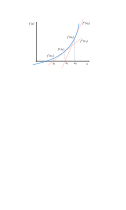
\includegraphics{figures/newton_method}
  \caption{Geometric interpretation of the Newton method in one dimension for an example function \(f\), whose derivative is denoted by \(f'\).}
  \label{fig:newton_method}
\end{figure}

In particular, using \(\pazocal R_\mathrm{J}\), a few simplifications can be obtained.
To ease the explanation, consider, a thermal residual operator $\pazocal{R}_{u}(\mathbf{u}, \bm{\uptheta})$ and a mechanical residual operator $\pazocal{R}_{\theta}(\mathbf{u}, \bm{\uptheta})$ defined to be the first and second components in the definition of \(\pazocal R_\mathrm{J}\) (Equation~\eqref{eq:def_res_gauss_seidel}).
Written in full
\begin{gather}
\pazocal{R}_{u}(\mathbf{u}, \bm{\uptheta})=\mathbf{u}-\pazocal{U}(\bm{\uptheta})=0, \\
\pazocal{R}_{\theta}(\mathbf{u}, \bm{\uptheta})=\bm{\uptheta}-\pazocal{T}(\mathbf{u})=0,
\end{gather}

From this, a block Newton iteration can be written as
\begin{highlight}
  \begin{equation} \label{eq:block_newton_raphson}
  \left[\begin{array}{l}
  J_{\pazocal{R}_{u}}\left(\mathbf u^k, \bm{\uptheta}^{k}\right) \\[7pt] J_{\pazocal{R}_{\theta}}\left(\mathbf{u}^{k}, \bm\uptheta^k\right)
  \end{array}\right]
  \left\{\begin{array}{c}\Delta \mathbf{u}^{k} \\ \Delta \bm{\uptheta}^{k}\end{array}\right\}
  =-\left\{\begin{array}{l}\pazocal{R}_{u}\left(\mathbf{u}^{k}, \boldsymbol{\theta}^{k}\right) \\ \pazocal{R}_{\theta}\left(\mathbf{u}^{k}, \boldsymbol{\theta}^{k}\right)\end{array}\right\},
  \end{equation}
\end{highlight}
and the update of the iteration variables reads
\begin{highlight}
  \begin{equation}
  \left\{\begin{array}{l}
  \mathbf{u}^{k+1} \\
  \boldsymbol{\theta}^{k+1}
  \end{array}\right\}=\left\{\begin{array}{l}
  \mathbf{u}^{k} \\
  \boldsymbol{\theta}^{k}
  \end{array}\right\}+\left\{\begin{array}{c}
  \Delta \mathbf{u}^{k} \\
  \Delta \boldsymbol{\theta}^{k}
  \end{array}\right\}.
  \end{equation}
\end{highlight}

The system of equations in Equation~\eqref{eq:block_newton_raphson} can be further simplified following \cite{degroote_development_2010} considering the definitions of the mechanical and thermal residuals and taking their derivatives.
It yields
\begin{equation}
\left[\begin{array}{cc}
\mathbf I & -J_{\pazocal{U}}\left(\bm{\uptheta}^{k}\right) \\[7pt]
-J_{\pazocal{T}}\left(\mathbf{u}^{k}\right) & \mathbf I
\end{array}\right]
\left\{\begin{array}{c}\Delta \mathbf{u}^{k} \\ \Delta \bm{\uptheta}^{k}\end{array}\right\}
=-\left\{\begin{array}{l}\pazocal{R}_{u}\left(\mathbf{u}^{k}, \boldsymbol{\theta}^{k}\right) \\ \pazocal{R}_{\theta}\left(\mathbf{u}^{k}, \boldsymbol{\theta}^{k}\right)\end{array}\right\},
\end{equation}

Solving for \(\Delta \mathbf u^k\) and \(\Delta \bm \uptheta^k\), one finds
\begin{align}
  \left(\mathbf I + J_\pazocal{U}(\bm\uptheta^k)J_\pazocal{T}(\mathbf u^k)\right)\Delta \mathbf u^k &= - \pazocal R_u(\mathbf u^k, \bm \uptheta^k)+J_\pazocal{U}(\bm\uptheta^k)\pazocal R_\theta(\mathbf u^k, \bm\uptheta^k), \label{eq:explicit_eq_delta_u_newton}\\
  \left(\mathbf I + J_\pazocal{T}(\mathbf u^k)J_\pazocal{U}(\bm\uptheta^k)\right)\Delta \bm\uptheta^k &= - \pazocal R_\theta(\bm \uptheta^k, \mathbf u^k)+J_\pazocal{\theta}(\mathbf u^k)\pazocal R_u(\mathbf u^k, \bm\uptheta^k). \label{eq:explicit_eq_delta_theta_newton}
\end{align}
Thus, the Jacobians now needed are \(J_\pazocal{U}\) and \(J_\pazocal{T}\).
See Section~\ref{sec:multisecant} for the practical application of this.

Every iteration of the Newton scheme involves at least one invocation of the thermal and mechanical solvers when computing $\pazocal{R}\left(\mathbf{u}^{k}\right)$ or both $\pazocal{R}_{u}\left(\mathbf{u}^{k}, \boldsymbol{\theta}^{k}\right)$ and $\pazocal{R}_{\theta}\left(\mathbf{u}^{k}, \boldsymbol{\theta}^{k}\right)$.
The critical point for black-box equation coupling is how to obtain the derivative information in the Jacobi matrices.
In different ways, some of the methods presented next find approximations for the required Jacobian times vector products.



\subsection{Constant Underrelaxation} \label{sec:underrelaxation}

One of the most straightforward ways to stabilize an iterative method is to use constant underrelaxation \citep{gatzhammer_efficient_2014}.
The relaxation is performed as follows
\begin{equation} \label{eq:constant_relaxation}
\mathbf x^{k+1}=(1-\omega) \mathbf x^{k}+\omega\left(\mathbf x^k - \pazocal R(\mathbf x^k)\right)=\mathbf x^{k} -\omega \pazocal R(\mathbf x^k),
\end{equation}
where \(\omega\) is the relaxation factor chosen in the range \(0<\omega<1\), which corresponds to an underrelaxation, to achieve a stabilizing effect.

Applying to Equation~\eqref{eq:def_res_jacobi}
\begin{equation}
  \left\{\begin{array}{c}
    \mathbf u^{k+1}\\
    \bm \uptheta^{k+1}
  \end{array}\right\} =
  (1-\omega)
  \left\{\begin{array}{c}
    \mathbf u^{k}\\
    \bm \uptheta^{k}
  \end{array}\right\}
  + \omega
  \left\{\begin{array}{c}
    \pazocal U(\bm\uptheta^k)\\
    \pazocal T(\mathbf u^k)
  \end{array}\right\}
\end{equation}
Applying to Equation~\eqref{eq:def_res_gauss_seidel}
\begin{equation}
  \bm\uptheta^{k+1} = (1-\omega)\bm\uptheta^k + \omega \pazocal T\circ\pazocal U(\bm \uptheta^k).
\end{equation}


Constant underrelaxation works well if \(\omega\) is close to 1 but leads to a slow convergence if \(\omega\) has to be chosen close to 0.
Thus, the constant underrelaxation method creates unmanageable computational costs for severe instabilities.
Overrelaxation can also be considered, keeping in mind that for \(\omega > 2\) convergence is lost.
The optimal \(\omega\) is not necessary the largest stable one \citep{gatzhammer_efficient_2014} and has to be set empirically.
In what follows, alternative methods are discussed to decrease the number of iterations necessary while maintaining stability.

\begin{framedbox}[htb]
  \caption{Constant underrelaxation applied to the block Gauss-Seidel scheme.}
  \label{box:constant_underrelaxation}
  \begin{center}
    \begin{minipage}{0.9\textwidth}
    \begin{enumerate}[(i)]
    \item \(\bm\uptheta^0 = \bm\uptheta_{n+1}^p\)
    \item Set fixed-point counter to zero: \(k=0\)
    \item Enter the fixed-point loop
    \begin{enumerate}[(1)]
      \item Solve the mechanical problem at fixed temeperature \(\bm \uptheta^k\): \(\mathbf u^{k+1} = \pazocal U(\bm \uptheta^k)\)
      \item Solve the thermal problem at a fixed configuration \(\mathbf u^{k+1}\): \(\bm \uptheta^{k+1} = \pazocal T(\mathbf u^{k+1})\)
      \item Compute \(\bm \uptheta^{k+1}\) using constant relaxation (Equation~\eqref{eq:constant_relaxation})
      \item If the desired accuracy has not been reached, update \(k=k+1\) and go to step (1).
    \end{enumerate}
    \end{enumerate}
    \end{minipage}
  \end{center}
\end{framedbox}

\section{One-point iteration function with memory}

\subsection{Aitken relaxation} \label{sec:aitken_relaxation}


The so-called Aitken \(\Delta^2\) relaxation method was introduced by \cite{irons_version_1969} as a modified Aitken \(\Delta^2\) that does not require the computation of the function twice per iteration as in the original method.
It has been widely used in the context of FSI \citep{irons_version_1969, kuttler_fixed-point_2008, joosten_analysis_2009, kuttler_vector_2009, erbts_partitioned_2015, wendt_partitioned_2015}.
It has also been used in the context of thermo-mechanics by \cite{danowski_monolithic_2013}.

In the one-dimensional case, this method resembles the secant method applied to the fixed point problem, which can be used to solve nonlinear equations without differentiation.
Calling it an Aitken method is perhaps a misnomer since, in the Aitken-Steffensen method, the function values are computed twice per iteration (see Section~\ref{sec:vector_extrapolation}).
It is more closely related to secant methods, reusing values from previous iterations.
This version of Aitken's \(\Delta^2\) method provides a dynamic under relaxation, which can be used to improve the convergence/stability properties of the coupling algorithm.

Assume that \(f\) is the function whose fixed point is sought.
The linear interpolation between two points already known of the function, \((a, f(a))\) and \((b, f(b)\) is
\begin{equation}
  y = \frac{f(b)-f(a)}{b-a}(x-a) + f(a).
\end{equation}
The fixed point of this approximation is
\begin{equation}
  c = \frac{f(b)-f(a)}{b-a}(c-a) + f(a).
\end{equation}
Thus, after rearranging,
\begin{equation}\
c=\frac{a f(b)- b f(a)}{\left(a-f(a)\right)-\left(b-f(b)\right)}
\end{equation}
This can be rewritten as
\begin{equation}
c=\left(1-\omega_{b}\right) b+\omega_{b} f(b) \quad \text { with } \omega_{b}=\frac{a-b}{\left(a-f(a)\right)-\left(b-f(b)\right)}
\end{equation}

Anticipating the next iteration step,
\begin{equation}
d=\left(1-\omega_{c}\right) c+\omega_{c} f(c) \quad \text { with } \omega_{c}=\frac{c-b}{\left(b-f(b)\right)-\left(c-f(c)\right)}
\end{equation}
a convenient expression for updating the relaxation factor may be found, i.e.
\begin{equation}
\omega_{c}=-\omega_{b}\frac{f(b)-b}{(c-f(c))-(f(b)-b)}.
\end{equation}
See Figure~\ref{fig:mod_aitken} for its geometric interpretation in one dimension.

\begin{figure}[htbp]
  \includegraphics{figures/mod_aitken}
  \caption{Geometric interpretation of the Aitken relaxation in one dimension for an example function \(f\) and corresponding interpreation as the secant method.}
  \label{fig:mod_aitken}
\end{figure}

Now, for the vector case, the next step is to work out the solution to the current iteration from the outcome of the previous iteration $\mathbf{x}^{k}$ plus a new increment $\Delta \mathbf{x}^{k}$
\begin{equation}
\mathbf{x}^{k+1}=\mathbf{x}^{k}+\Delta \mathbf{x}^{k}.
\end{equation}
The increment reads
\begin{equation} \label{eq:aitken_update}
\Delta \mathbf{x}^{k}=\omega^{k}\left(\pazocal S(\mathbf{x}^{(k)})-\mathbf{x}^{(k)}\right)=-\omega^{k} \pazocal R(\mathbf x^k).
\end{equation}
with $\omega^{k}$ being the relaxation coefficient.
This coefficient is updated in every iteration cycle as a function of two previous residuals
\begin{highlight}
  \begin{equation} \label{eq:aitken_relaxation_factor}
    \omega^{k}=-\omega^{k-1} \frac{\left(\mathbf{r}^{(k)}-\mathbf{r}^{(k-1)}\right)^{\mathrm{T}} \mathbf{r}^{(k-1)}}{\left(\mathbf{r}^{(k)}-\mathbf{r}^{(k-1)}\right)^{2}}.
  \end{equation}
\end{highlight}
Comparing with Equations~\eqref{eq:newton_system} and \eqref{eq:newton_iter}, \(\omega^{k}\) can be, in a sense, regarded as an approximation to the inverse of the Jacobian.
Dynamic relaxation is also easy to implement, and the additional computational input is acceptable since only inner vector products must be performed.
The dynamical relaxation coefficient is restricted to the range \((0,2)\) because employing relaxation with a relaxation coefficient outside this range leads to loss of convergence \citep{erbts_accelerated_2012}.
See Box~\ref{box:aitken_relaxation} for the pseudocode.

\begin{framedbox}[htb]
  \caption{Aitken relaxation for one timestep.}
  \label{box:aitken_relaxation}
  \begin{center}
    \begin{minipage}{0.9\textwidth}
    \begin{enumerate}[(i)]
    \item Set nonlinear counter to zero: \(k=0\)
    \item \(\mathbf x^k = \mathbf x_{n+1}^p\)
    \item Enter the nonlinear loop
    \begin{enumerate}[(1)]
      \item Compute \(\pazocal R(\mathbf x^k)\), which implies the solution of the mechanical and the thermal problems, \(\pazocal U\) and \(\pazocal T\), respectively.
      \item if \(k=0\):
      \begin{itemize}
        \item Compute \(\mathbf x^{k+1}\) using constant relaxation (Equation~\eqref{eq:constant_relaxation})
      \end{itemize}
      \item else:
      \begin{itemize}
        \item Compute \(\mathbf x^{k+1}\) using Aitken relaxation relaxation (Equations~\eqref{eq:aitken_update} and \eqref{eq:aitken_relaxation_factor})
        \item Save the current residue \(\mathbf r^k = \pazocal R^k\).
      \end{itemize}
      \item If the desired accuracy has not been reached, update \(k=k+1\) and go to step (1).
    \end{enumerate}
    \end{enumerate}
    \end{minipage}
  \end{center}
\end{framedbox}

\subsection{Multi-secant methods} \label{sec:multisecant}

The following exposition follows closely \cite{fang_two_2009}.
In quasi-Newton methods the Jacobian is updated in each iteration using a rank-one update.
Standard quasi-Newton methods require the updated \(J_{k+1}\) to satisfy the following secant condition
\begin{equation} \label{eq:secant_condition}
J_\pazocal{R}^{k+1} \Delta \mathbf x^{k}=\Delta \pazocal R^{k},
\end{equation}
where \(\Delta \pazocal R^{k}\equiv \pazocal R\left(\mathbf x^{k+1}\right)-\pazocal R\left(\mathbf x^ {k}\right)\).
Furthermore, another common requirement is the following so-called no-change condition
\begin{equation} \label{eq:no_change_condition}
J_\pazocal R^{k+1} \mathbf q=J_\pazocal R^{k} \mathbf q \quad \forall \mathbf q \text { such that } \mathbf q^{\mathrm{T}} \Delta \mathbf x^{k}=0,
\end{equation}
which stipulates that there be no new information from \(J_\pazocal R^{k}\) to \(J_\pazocal R^{k+1}\) along any direction \(\mathbf q\) orthogonal to \(\Delta \mathbf x^{k}\).

\cite{broyden_class_1965} developed a method satisfying both secant condition (Equation~\eqref{eq:secant_condition}) and the no-change condition (Equation~\eqref{eq:no_change_condition}), arriving at the update formula
\begin{highlight}
\begin{equation} \label{eq:good_update_broyden}
J_{\pazocal R}^{k+1}=J_{\pazocal R}^{k}+\left(\Delta \pazocal R^{k}-J_{\pazocal R}^{k} \Delta \mathbf x^{k}\right) \frac{\Delta {\mathbf x^{k}}^{\mathrm{T}}}{\Delta {\mathbf x^{k}}^{\mathrm{T}} \Delta \mathbf x^{k}}.
\end{equation}
\end{highlight}

Matrix \(J_\pazocal R^{k+1}\) in Equation~\eqref{eq:good_update_broyden} is the unique matrix satisfying both conditions \eqref{eq:secant_condition} and \eqref{eq:no_change_condition}.
The Broyden update can also be obtained by minimizing \(E\left(J_\pazocal R^{k+1}\right)=\left\|J_\pazocal R^{k+1}-J_\pazocal R^{k}\right\|_{F}^{2}\) with respect to terms of \(J_\pazocal R^{k+1}\), subject to the secant condition \eqref{eq:secant_condition}.

It may seem at first that Broyden's first method can be expensive since computing the quasi-Newton step \(\Delta \mathbf x^{k}\) requires solving a linear system at each iteration.
However, note that, typically, the approximate Jacobian is a small rank modification of a diagonal matrix (or a matrix that is easy to invert); hence, the cost to obtain this solution is not too high as long as the number of steps is not too large.

An alternative is Broyden's second method that approximates the inverse Jacobian instead of the Jacobian itself.
\(G_\pazocal R^{k}\) is used to denote the estimated inverse Jacobian at the \(k\) th iteration.
The secant condition (Equation~\eqref{eq:secant_condition}) now reads
\begin{equation} \label{eq:inverse_secant_cond}
G_\pazocal R^{k+1} \Delta \pazocal R^{k}=\Delta \mathbf x^{k}
\end{equation}
By minimizing \(E\left(G_\pazocal R^{k+1}\right)=\left\|G_\pazocal R^{k+1}-G_\pazocal R^{k}\right\|_{F}^{2}\) with respect to \(G_\pazocal R^{k+1}\) subject to Equation~\eqref{eq:inverse_secant_cond}, the following update formula is found for the inverse Jacobian
\begin{highlight}
  \begin{equation} \label{eq:bad_update_broyden}
  G_\pazocal R^{k+1}=G_\pazocal R^{k}+\left(\Delta \mathbf x_{k}-G_\pazocal R^{k} \Delta \pazocal R^{k}\right) \frac{\Delta {\pazocal R^{k}}^{\mathrm{T}}}{\Delta {\pazocal R^{k}}^{\mathrm{T}} \Delta \pazocal R^{k}}
  \end{equation}
\end{highlight}
which is also the only update satisfying both the secant condition (Equation~\eqref{eq:inverse_secant_cond}) and the no-change condition for the inverse Jacobian
\begin{equation}
  G_\pazocal R^{k} \mathbf q=G_\pazocal R^{k+1} \mathbf q \quad \forall \mathbf q \text { such that } \mathbf q^{\mathrm{T}} \Delta \pazocal R^{k}=0.
\end{equation}
The update formula in Equation~\eqref{eq:good_update_broyden} can also be obtained in terms of \(G_\pazocal R^{k} \equiv {J_\pazocal R^{k}}^{-1}\) by applying the Sherman-Morrison formula
\begin{equation} \label{eq:g_broyden_type_i}
G_\pazocal R^{k+1}=G_\pazocal R^{k}+\left(\Delta \mathbf x^{k}-G_\pazocal R^{k} \Delta \pazocal R^{k}\right) \frac{\Delta {\mathbf x^{k}}^{\mathrm{T}} G_\pazocal R^{k}}{\Delta {\mathbf x^{k}}^{\mathrm{T}} G_\pazocal R^{k} \Delta \pazocal R^{k}}
\end{equation}
This shows, as was explained earlier, that to solve the Jacobian system associated with Broyden's first approach can be reduced to a set of update operations that are not more costly than those required by the second update.
Note, however, that the above formula requires the inverse of the initial Jacobian.

From Equation~\eqref{eq:good_update_broyden} and Equation~\eqref{eq:bad_update_broyden} it is possible to define Broyden's family of updates, in which an update formula takes the general form
\begin{equation}
G_\pazocal R^{k+1}=G_\pazocal R^{k}+\left(\Delta \mathbf x^{k}-G_\pazocal R^{k} \Delta \pazocal R^{k}\right) \mathbf v_{k}^{\mathrm{T}}
\end{equation}
where \(\mathbf v_{k}^{\mathrm{T}} \Delta \pazocal R^{k}=1\) so that the secant condition \eqref{eq:secant_condition} holds.
Note that the secant condition \eqref{eq:inverse_secant_cond} is equivalent to condition \eqref{eq:secant_condition}.
% The pseudocode of Broyden's two methods is given in Box~\ref{box:broydens_method}.
Some authors called Broyden's first method Broyden's good update and Broyden's second method as Broyden's bad update.
These are two particular members of Broyden's family.

% \begin{framedbox}[htb]
%   \caption{Broyden's method for one timestep.}
%   \label{box:broydens_method}
%   \begin{center}
%     \begin{minipage}{0.9\textwidth}
%     \begin{enumerate}[(i)]
%     \item Set nonlinear counter to zero: \(k=0\)
%     \item \(\mathbf x^k = \mathbf x_{n+1}^p\)
%     \item Evaluate \(\pazocal R^k = \pazocal R(\mathbf x^k)\), which implies the solution of the mechanical and the thermal problems, \(\pazocal U\) and \(\pazocal T\), respectively.
%     \item Enter the nonlinear loop
%     \begin{enumerate}[(1)]
%       \item Compute the update step from \(\Delta \mathbf x^k = - G^k_\pazocal R \pazocal R^k\),
%       \item Update \(\mathbf x^{k+1} = \mathbf x^k + \Delta \mathbf x^k\),
%       \item Evaluate \(\pazocal R^{k+1} = \pazocal R(\mathbf x^{k+1})\), which implies the solution of the mechanical and the thermal problems, \(\pazocal U\) and \(\pazocal T\), respectively.
%       \item Compute \(\Delta \pazocal R^k = \pazocal R^{k+1} - \pazocal R^k\).
%       \item if the first update is to be used:
%       \begin{itemize}
%         \item Set \({{\mathbf{v}}^k}^T = \Delta {\mathbf x^k}^T G^k_\pazocal R\),
%       \end{itemize}
%       \item else if the second update is to be used:
%       \begin{itemize}
%         \item Set \({{\mathbf{v}}^k}^T = \Delta {\pazocal R^k}^T\),
%       \end{itemize}
%       \item \(G_\pazocal R^{k+1} = G_\pazocal R^k + (\Delta \mathbf x^k - G_\pazocal R^k\Delta \pazocal R^k)\frac{{{\mathbf{v}}^k}^T}{{{\mathbf{v}}^k}^T\Delta \pazocal R^k}.\)
%       \item If the desired accuracy has not been reached, update \(k=k+1\) and go to step (1).
%     \end{enumerate}
%     \end{enumerate}
%     \end{minipage}
%   \end{center}
% \end{framedbox}


\subsubsection{Generalized Broyden}

The multi-secant methods provide an approximation to the Jacobian in Equation~\eqref{eq:newton_system} or Equation~\eqref{eq:block_newton_raphson} using information from previous iterations.
A generalized Broyden's method with a flexible rank update on the inverse Jacobian, satisfying a set of \(m\) secant equations
\begin{equation} \label{eq:multi_secant_eqs}
  G_\pazocal R^{k} \Delta \pazocal R^{i}=\Delta \mathbf x^{i} \quad \text { for } i=k-m, \ldots, k-1
\end{equation}
where it is assumed \(\Delta \pazocal R^{k-m}, \ldots, \Delta \pazocal R^{k-1}\) are linearly independent and \(m \leqslant n\) can also be described.
Aggregating Equations~\eqref{eq:multi_secant_eqs} in matrix form, they can be rewriten it as
\begin{equation} \label{eq:multi_secant_eqs_mat}
  G_\pazocal R^{k} \mathscr{R}^{k}=\mathscr{X}^{k}.
\end{equation}
where
\begin{equation}
\mathscr{R}^{k}=\left[\Delta \pazocal R^{k-m} \cdots \Delta \pazocal R^{k-1}\right], \quad \mathscr{X}^{k}=\left[\Delta \mathbf x^{k-m} \cdots \Delta \mathbf x^{k-1}\right] \in \mathbb{R}^{n \times m}
\end{equation}
The no-change condition corresponding to \eqref{eq:no_change_condition} is
\begin{equation}
  \left(G_\pazocal R^{k}-G_\pazocal R^{k-m}\right) \mathbf q=0
\end{equation}
for all \(\mathbf q\) orthogonal to the subspace spanned by \(\Delta \pazocal R^{k-m}, \ldots, \Delta \pazocal R^{k-1}\), the columns of \(\mathscr{R}^{k}\).
In the end, this yields
\begin{equation}
  G_\pazocal R^{k}=G_\pazocal R^{k-m}+\left(\mathscr{X}^{k}-G_\pazocal R^{k-m} \mathscr{R}^{k}\right)\left({\mathscr{R}^{k}}^{\mathrm{T}} \mathscr{R}^{k}\right)^{-1} {\mathscr{R}^{k}}^{\mathrm{T}}
\end{equation}
a rank-\(m\) update formula.
Note that \(\operatorname{rank}\left(\mathscr{R}^{k}\right)=m\).
The update formula for \(\mathbf x^{k+1}\) is
\begin{align}
\mathbf x^{k+1} &=\mathbf x^{k}-G_\pazocal R^{k} \pazocal R^{k} \\
&=\mathbf x^{k}-G_\pazocal R^{k-m} \pazocal R^{k}-\left(\mathscr{X}^{k}-G_\pazocal R^{k-m} \mathscr{R}^{k}\right)\left({\mathscr{R}^{k}}^{\mathrm{T}} \mathscr{R}^{k}\right)^{-1} {\mathscr{R}^{k}}^{\mathrm{T}} \pazocal R^{k} \\
&=\mathbf x^{k}-G_\pazocal R^{k-m} \pazocal R^{k}-\left(\mathscr{X}^{k}-G_\pazocal R^{k-m} \mathscr{R}^{k}\right) \gamma_{k} \label{eq:update_gen_broyden_ls}
\end{align}
where the column vector \(\gamma_{k}\) is obtained by solving the normal equations \(\left({\mathscr{R}^{k}}^{\mathrm{T}} \mathscr{R}^{k}\right) \gamma_{k}={\mathscr{R}^{k}}^{\mathrm{T}} \pazocal R^{k}\), which is equivalent to solving the least squares problem
\begin{equation}
  \min _{\gamma}\left\|\mathscr{R}^{k} \gamma-\pazocal R^{k}\right\|_{2}.
\end{equation}
Note that in Equation~\eqref{eq:update_gen_broyden_ls}, if \(\mathscr{R}^{k}\) is square and of full rank, then for any \(G_\pazocal R^{k-m}\),
\begin{equation}
  \mathbf x^{k+1}=\mathbf x^{k}-\mathscr{X}^{k} {\mathscr{R}^{k}}^{-1} \pazocal R^{k},
\end{equation}
the same form as that in the standard secant method.

\subsubsection{Anderson mixing}

The Anderson mixing scheme [5] takes the latest \(m\) steps into account to obtain a better approximation to \(\mathbf x_{n+1}\) without evaluating \(\pazocal R\) again.
Consider
\begin{align}
  \bar{\mathbf x}^{k}=\mathbf x^{k}-\sum_{i=k-m}^{k-1} \gamma_{i}^{k} \Delta \mathbf x^{i}=\mathbf x_{k}-\mathscr{X}^{k} \gamma^{k}, \label{eq:anderson_x_bar}\\
  \bar{\pazocal R}^{k}=\pazocal R^{k}-\sum_{i=k-m}^{k-1} \gamma_{i}^{k} \Delta \pazocal R^{i}=\pazocal R^{k}-\mathscr{R}^{k} \gamma^{k} \label{eq:anderson_r_bar},
\end{align}
where \(\Delta \mathbf x^{i}=\mathbf x^{i+1}-\mathbf x^{i}\) and \(\Delta \pazocal R^{i}=\pazocal R^{i+1}-\pazocal R^{i}\), \(\mathscr{X}^{k}=\left[\Delta \mathbf x^{k-m} \cdots \Delta \mathbf x^{k-1}\right]\), \(\mathscr{R}^{k}=\left[\Delta \pazocal R^{k-m} \cdots \Delta \pazocal R^{k-1}\right]\), and \(\gamma^{k}=\left[\gamma_{k-m}^{k} \cdots \gamma_{k-1}^{k}\right]^{\mathrm{T}}\).
Expressing the equations in the form \(\bar{\mathbf x}^{k}=\sum_{j=k-m}^{k} w_{j} \mathbf x^{j}\) and \(\bar{\pazocal R}^{k}=\sum_{j=k-m}^{k} w_{j} \pazocal R^{j}\), it is found that \(\sum_{j=k-m}^{k} w_{j}=1\).
In other words, \(\bar{\mathbf x}_{k}\) and \(\bar{\pazocal R}_{k}\) are weighted averages of \(\mathbf x_{k-m}, \ldots, \mathbf x_{k}\) and \(\pazocal R^{k-m}, \ldots, \pazocal R^{k}\), respectively.
The arguments \(\gamma^{k}=\left[\gamma_{k-m}^{k} \cdots \gamma_{k-1}^{k}\right]^{\mathrm{T}}\) are determined by minimizing
\begin{equation}
E\left(\gamma^{k}\right)=\left\langle\bar{\pazocal R}^{k}, \bar{\pazocal R}^{k}\right\rangle=\left\|\pazocal R^{k}-\mathscr{R}^{k} \gamma^{k}\right\|_{2}^{2}
\end{equation}
whose solution can, but should not in practice, be obtained by solving the normal equations
\begin{equation}
\left({\mathscr{R}^{k}}^{\mathrm{T}} \mathscr{R}^{k}\right) \gamma^{k}={\mathscr{R}^{k}}^{\mathrm{T}} \pazocal R^{k}. \label{eq:normal_eqs_anderson}
\end{equation}
Combining Equations~\eqref{eq:anderson_x_bar}, \eqref{eq:anderson_r_bar}, and \eqref{eq:normal_eqs_anderson}, one obtains
\begin{align}
\mathbf x^{k+1} &=\bar{\mathbf x}^{k}+\beta \bar{\pazocal R}^{k} \\
&=\mathbf x^{k}+\beta \pazocal R^{k}-\left(\mathscr{X}^{k}+\beta \mathscr{R}^{k}\right) \gamma^{k} \\
&=\mathbf x^{k}+\beta \pazocal R^{k}-\left(\mathscr{X}^{k}+\beta \mathscr{R}^{k}\right)\left({\mathscr{R}^{k}}^{\mathrm{T}} \mathscr{R}^{k}\right)^{-1} {\mathscr{R}^{k}}^{\mathrm{T}} \pazocal R^{k} \label{eq:update_anderson_mixing}
\end{align}
where \(\beta\) is the preset mixing parameter and \({\mathscr{R}^{k}}^{\mathrm{T}} \mathscr{R}^{k}\) is assumed to be nonsingular.
In particular, if no previous iterate is taken into account (i.e. \(m=0\) ), then Equation~\eqref{eq:update_anderson_mixing} reads
\begin{equation}
  \mathbf x^{k+1}=\mathbf x^{k}+\beta \pazocal R^{k}
\end{equation}
This scheme is referred to as simple mixing and underrelaxation if \(0<\beta<1\) (see Section~\ref{sec:underrelaxation}).
The update formula \eqref{eq:update_anderson_mixing} is the same as \eqref{eq:update_gen_broyden_ls} by setting \(G_\pazocal R^{k-m}=-\beta \mathbf I\).
In this respect Anderson mixing implicitly forms an approximate inverse Jacobian \(G_\pazocal R^{k}\) that minimizes \(\left\|G_\pazocal R^{k}+\beta \mathbf I\right\|_{F}\) subject to \eqref{eq:multi_secant_eqs_mat}.
In the context of mixing, generalized Broyden's second method is equivalent to Anderson mixing.
Note that if \(\mathscr{R}^{k}\) is square and nonsingular, then Equation~\eqref{eq:update_anderson_mixing} matches the formula of the standard secant method.

\subsubsection{Generalized Broyden's family} \label{sec:gen_broyden_fam}

Now we can write down the generalized Broyden family, in which an update algorithm is in the form
\begin{equation} \label{eq:inv_jacob_gen_broyden}
G_\pazocal R^{k}=G_\pazocal R^{k-m}+\left(\mathscr{X}^{k}-G_\pazocal R^{k-m} \mathscr{R}^{k}\right) {V^{k}}^{\mathrm{T}}
\end{equation}
where \({V^{k}}^{\mathrm{T}} \mathscr{R}^{k}=I\) so that the secant condition \(G_\pazocal R^{k} \mathscr{R}^{k}=\mathscr{X}^{k}\) holds.
The two optimal choices of \({V^k}^T = {M^k}^{-1}{N^k}^T\) are
\begin{equation} \label{eq:broyden_type_ii}
  {M^k} = {\mathscr R^k}^T \mathscr R^k,\quad {N^k}^T = {\mathscr R^k}^T,
\end{equation}
minimizaing \(\left\|G_\pazocal R^k - G_\pazocal R^{k-m}\right\|_F\) and
\begin{equation} \label{eq:broyden_type_i}
  {M^k} = {\mathscr X^k}^T G_\pazocal R^k \mathscr R^k,\quad {N^k}^T = {\mathscr X^k}^T G_\pazocal R^k,
\end{equation}
minimizaing \(\left\|J_\pazocal R^k - J_\pazocal R^{k-m}\right\|_F\).
This last choice yields as the approximation for the Jacobian
\begin{equation}
  J_\pazocal R^{k}=J_\pazocal R^{k-m}+\left(\mathscr{R}^{k}-J_\pazocal R^{k-m} \mathscr{X}^{k}\right)\left({\mathscr{X}^{k}}^{\mathrm{T}} \mathscr{X}^{k}\right)^{-1} {\mathscr{X}^{k}}^{\mathrm{T}},
\end{equation}
after applying the Woodbury formula.
The first choice is said to correspond to a Type-II update and the second to a Type-I update \citep{fang_two_2009}.

% \begin{framedbox}[htb]
%   \caption{Generalized Broyden's family method for one timestep.}
%   \label{box:broydens_method}
%   \begin{center}
%     \begin{minipage}{0.9\textwidth}
%     \begin{enumerate}[(i)]
%     \item Set nonlinear counter to zero: \(k=0\)
%     \item Set \(\mathbf x^k = \mathbf x_{n+ 1}^p\) and choose an initial estimate for \(\mathbf G_1 = J^{-1}_\pazocal R(\mathbf x^k)\).
%     \item Evaluate \(\pazocal R^k = \pazocal R(\mathbf x^k)\), which implies the solution of the mechanical and the thermal problems, \(\pazocal U\) and \(\pazocal T\), respectively.
%     \item Enter the nonlinear loop
%     \begin{enumerate}[(1)]
%       \item Compute the update step from \(\Delta \mathbf x^k = - G^k_\pazocal R \pazocal R^k\) and add it to \(\mathscr X^k\). If the maximum number of previous iteration \(m\) replace the oldest column.
%       \item Update \(\mathbf x^{k+1} = \mathbf x^k + \Delta \mathbf x^k\),
%       \item Evaluate \(\pazocal R^{k+1} = \pazocal R(\mathbf x^{k+1})\), which implies the solution of the mechanical and the thermal problems, \(\pazocal U\) and \(\pazocal T\), respectively.
%       \item Compute \(\Delta \pazocal R^k = \pazocal R^{k+1} - \pazocal R^k\) and add it to \(\mathscr R^k\). If the maximum number of previous iteration has been reach replace the oldest column.
%       \item Compute \({\mathbf V^k}^T\) according to the type of update chosen (Equation~\eqref{eq:broyden_type_i} and \eqref{eq:broyden_type_ii}).
%       \item \(G_\pazocal R^{k+1} = G_\pazocal R^k + (\mathscr X^k - G_\pazocal R^k\mathscr R^k){{\mathbf{V}}^k}^T.\)
%       \item If the desired accuracy has not been reached, update \(k=k+1\) and go to step (1).
%     \end{enumerate}
%     \end{enumerate}
%     \end{minipage}
%   \end{center}
% \end{framedbox}

\subsubsection{Anderson's family}

The udpate formula for Anderson's family can be found from Equation~\eqref{eq:inv_jacob_gen_broyden} using as the approximation to the previous Jacobian the identity matrix multiplied by a constant \(\beta\), i.e.,
\begin{equation} \label{eq:andersons_family_update}
  \mathbf x^{k+1} = \mathbf x^{k} + \beta \pazocal R^k - (\mathscr X^k + \beta\mathscr R^k){\mathbf V^k}^T \pazocal R^k.
\end{equation}
The two choices for \(\mathbf V^k\) remain the same, replacing \(G_\pazocal R^{k-m}\) by \(-\beta\mathbf I\).
They now minimize \(\|G_\pazocal R^k+\beta\mathbf I\|\) and \(\|J_\pazocal R^k + (1/\beta)\mathbf I\|\).

% \begin{framedbox}[htb]
%   \caption{Anderson's family method for one timestep.}
%   \label{box:broydens_method}
%   \begin{center}
%     \begin{minipage}{0.9\textwidth}
%     \begin{enumerate}[(i)]
%     \item Set \(\mathbf x^0 = \mathbf x_{n+ 1}^p\).
%     \item Evaluate \(\pazocal R^0 = \pazocal R(\mathbf x^k)\), which implies the solution of the mechanical and the thermal problems, \(\pazocal U\) and \(\pazocal T\), respectively.
%     \item Compute \(\mathbf x^1 = \mathbf x^0 + \beta R^0\).
%     \item Evaluate \(\pazocal R^{1} = \pazocal R(\mathbf x^{1})\), which implies the solution of the mechanical and the thermal problems, \(\pazocal U\) and \(\pazocal T\), respectively.
%     \item Set nonlinear counter to zero: \(k=1\)
%     \item Enter the nonlinear loop
%     \begin{enumerate}[(1)]
%       \item Compute \(\Delta \pazocal R^{k-1} = \pazocal R^{k} - \pazocal R^{k-1}\) and add it to \(\mathscr R^k\).
%       If the maximum number of previous iteration has been reached either replace the oldest column or restart \(\mathscr R^k\).
%       \item Compute \(\Delta \mathbf x^{k-1} = \mathbf x^{k} -\mathbf x^{k-1} \) and add it to \(\mathscr X^k\).
%         If the maximum number of previous iteration has been reached either replace the oldest column or restart \(\mathscr X^k\).
%       \item Compute \({\mathbf V^k}^T\) according to the type of update chosen (Equation~\eqref{eq:broyden_type_i} and \eqref{eq:broyden_type_ii}).
%       \item Update according to \(\mathbf x^{k+1} = \mathbf x^k + \beta \pazocal R^k + \left(\mathscr X^k + \beta\mathscr R^k\right){\mathbf V^k}^T\pazocal R^k \).
%       \item Evaluate \(\pazocal R^{k+1} = \pazocal R(\mathbf x^{k+1})\), which implies the solution of the mechanical and the thermal problems, \(\pazocal U\) and \(\pazocal T\), respectively.
%       \item If the desired accuracy has not been reached, update \(k=k+1\) and go to step (1).
%     \end{enumerate}
%     \end{enumerate}
%     \end{minipage}
%   \end{center}
% \end{framedbox}

\subsubsection{The Broyden-like class}

Both the generalized Broyden's family and Anderson's family can be understood as methods in the Broyden-like class as described in \cite{fang_two_2009}.
Ssuppose the latest \(m\) iterates are available, which are denoted by \(\mathbf x^{1}, \ldots, \mathbf x^{m}\).
Let \(\Delta \mathbf x^{i}=\mathbf x^{i+1}- \mathbf x^{i}\) for \(i=1, \ldots, m-1\).
Partition \(\Delta \mathbf x^{1}, \ldots, \Delta \mathbf x^{m-1}\) into \(p\) groups,
\begin{align}
\mathscr{X}^{1} & =\left[\Delta \mathbf x^{1}, \ldots, \Delta \mathbf x^{z_{1}}\right], \\
\mathscr{X}^{2} & =\left[\Delta \mathbf x^{z_{1}+1}, \ldots, \Delta \mathbf x^{z_{2}}\right],\\
& \vdots \\
\mathscr{X}^{p} & =\left[\Delta \mathbf x^{z_{k-1}+1}, \ldots, \Delta \mathbf x^{z_{k}}\right],
\end{align}
where \(z_{i}\) is the index of the last entry in the \(i\) th group for \(i=1, \ldots, p\); \(z_{0}=0\) and \(z_{p}=m-1\).
Also partition \(\Delta \pazocal R^{1}, \ldots, \Delta \pazocal R^{m-1}\) into \(\mathscr R^{1}, \ldots, \mathscr R^p\) accordingly, where \(\Delta \pazocal R^{i}=\pazocal R^{i+1}- \pazocal R^{i}\) with \(\pazocal R^{i}=\pazocal R(\mathbf x^{i})\).  The sizes of the groups for \(i=1, \ldots, k\) are denote by \(s_{i}:=z_{i}-z_{i-1}\).
Note that the indexing here is different from the previous sections.
The inverse of the Jacobian is iteratively approximated at the \(\left(z_{i}+1\right)\)st iterate for \(i=1, \ldots, p\) as
\begin{equation} \label{sec:broyden_like_class_g_update}
  G_\pazocal R^{i+1} = G_\pazocal R^{i}+\left(\mathscr{X}^{i}-G_\pazocal R^{i} \mathscr R^{i}\right) {\mathbf V^{i}}^T,
\end{equation}
where \({\mathbf V^{i}}^T \mathscr{R}^{i}=\mathbf I\) for the secant condition.
The update follows the formula of the generalized Broyden family.
In the context of mixing, the base case is
\begin{equation}
  G_\pazocal R^{1}=-\beta \mathbf I,
\end{equation}
where \(\beta\) is the mixing parameter.
The next iterate is set as
\begin{equation} \label{eq:update_broyden_family}
  \mathbf x^{m+1}=\mathbf x^{m}-G_\pazocal R^{k+1} \pazocal R^m.
\end{equation}
The choice of \(V_{i}\) satisfying \(V_{i}^{\mathrm{T}} \mathscr{F}_{i}=I\) is performed as described in Section~\ref{sec:gen_broyden_fam}.

\subsection{Practical considerations}

The application of Broyden's method as described so far is unfeasible for the problems considered in this document, i.e., thermo-mechanical coupled problems with many unknowns.
So far, the descriptions considered of the Broyden-like class methods require one to keep the large \(G_\pazocal R^i\) matrices of size \(n_\text{unknowns}\times n_\text{unknowns}\) in memory, in addition to the previous iterates.
This is a significant drawback.
However, \cite{fang_two_2009} present a more memory efficient way of implementing these methods.
Let
\begin{equation} \label{eq:def_e_broyden}
E^{i}=\mathscr{X}^{i}-G_\pazocal R^{i} \mathscr R^{i}.
\end{equation}
Substituting Equation~\eqref{eq:def_e_broyden} into Equation~\eqref{sec:broyden_like_class_g_update} one obtains
\begin{align}
  G_\pazocal R^{i}=& G_\pazocal R^{i-1}+E^{i-1} {V^{i-1}}^T, \\
  =& G_\pazocal R^{i-2} + E^{i-2} {V^{i-2}}^T + E^{i-1} {V^{i-1}}^T, \\
  & \vdots \\
  =& G_\pazocal R^{1}+\sum_{j=1}^{i-1} E^{j} {V^{j}}^{\mathrm{T}}, \label{eq:update_broyden_family_g_mem}
\end{align}
for \(i=2, \ldots, p+1\).
Matrices \(G_\pazocal R^{i}\) need not be explicitly stored.
\(G_\pazocal R^{i}\) is needed  only to compute \(G_\pazocal R^{i} \mathscr R^{i}\) in Equation~\eqref{eq:def_e_broyden} and \(G_\pazocal R^{p+1} \pazocal R^{m}\) in Equation~\eqref{eq:update_broyden_family}, and also for \(V^{i}\) if it depends on \(G_\pazocal R^{i}\).
Substituting Equation~\eqref{eq:update_broyden_family_g_mem} into Equation~\eqref{eq:def_e_broyden} obtains
\begin{equation} \label{eq:update_eq_for_e}
E^{i}=\mathscr{X}^{i}-G_\pazocal R^1 \mathscr{R}^{i}-\sum_{j=1}^{i-1} E^{j}\left({V^{j}}^T \mathscr{R}^{i}\right),
\end{equation}
for \(i=1, \ldots, p\).
The computation is economic for large-scale problems with \(n \gg m\).
The next iterate \(\mathbf x^{m+1}\) in (32) can also be computed in a similar manner
\begin{equation} \label{eq:mem_eff_update_broyden}
  \mathbf x^{m+1}=\mathbf x^{m} - G_\pazocal R^{p+1} \pazocal R^{m}= \mathbf x^{m} - G_\pazocal R^1 \pazocal R^{m}-\sum_{j=1}^{k} E^{j}\left({V^{j}}^T \pazocal R^m\right).
\end{equation}

Using Type-II update, the computation of \(V^{i}\) is straightforward from \(\mathscr{R}^{i}\).
On the other hand, Type-I update involves \(G_\pazocal R^{i}\) to compute \(V^{i}\).
Thus
\begin{equation} \label{eq:compute_n_broyden}
  {N^{i}}^T={\mathscr{X}^{i}}^T G_\pazocal R^{i}=G_\pazocal R^1 {\mathscr{X}^{i}}^T+\sum_{j=1}^{i-1}\left({\mathscr{X}^{i}}^{\mathrm{T}} E^{j}\right) {V^{j}}^T.
\end{equation}
After obtaining \(N^{i}\), we compute \(M^{i}={N^{i}}^T \mathscr{R}^{i}\) and then \({V^{i}}^T={M^{i}}^{-1} {N^{i}}^T\) for \(i=1, \ldots, p\).

Looking at Equations~\eqref{eq:update_eq_for_e}, \eqref{eq:mem_eff_update_broyden} and \eqref{eq:compute_n_broyden}, one still needs the initial approximation to the inverse of the Jacobian, \(G_\pazocal R^1\), whose size is \(n_\text{unknown}\times n_\text{unknown}\).
In \cite{fang_two_2009} the approach adopted was to follow the idea of Anderson's mixing and set
\begin{equation}
  G_\pazocal R^1 = - \beta \mathbf I,
\end{equation}
drastically improving the memory requirements, as only one scalar parameter, \(\beta\), needs to be saved.
Also, \cite{kelley_solving_2003}, assumes in his implementation of Broyden's method, an initial approximation to \(G_\pazocal R^1\) equal to the identity matrix.
Information about \(G_\pazocal R^1\) is applied in the preconditioning of the system instead.

To compute \(V^i\), \cite{fang_two_2009} suggest a \(QR\) decomposition with pivoting.
Be it for a Type-II update, where one needs to solve a least-squares problem, or for a Type-I update, one needs to invert a generally non-symmetric matrix.
This approach leads to better numerical stability when the matrices to be inverted are singular or ill-conditioned, compared with solving the normal equations.
The \(QR\) decomposition has a computational cost of \(\pazocal O(n_\text{unknown}m^2)\) algebraic operations \citep{dennis_numerical_1996}.

If the size of the groups \(s_1, s_2,\dots\) are fixed from one Newton iteration to the next, so the \(E^i\) and \(V^i\) matrices remain the same from one iteration to the next, the computation effort to compute them is saved from one iteration to the next.
Here only constant \(s=s_1=s_2 =\cdots\) is considered, where \(s=\infty\) corresponds to Anderson's mixing, where all previous iterates available are considered.

One question remains. How to proceed when the available memory runs out?.
According to \cite{kelley_solving_2003}, as is often the case with GMRES, the iteration can be restarted if there is no more room to store the vectors.
A different approach, called limited memory in the optimization literature, is to replace the oldest of the stored steps with the most recent one.

Thus, appplying the method as suggest by \cite{fang_two_2009}, leads to a storage need of
\begin{enumerate}
  \item  Two column vectors of size \(n_\text{unknown}\) for \(\mathbf x^{m}\) and \(\pazocal R^{m}\).
  \item An \(n_\text{unknown} \times(m-1)\) matrix for \(\mathscr{X}^{1}, \ldots, \mathscr{X}^{k}\) (shared with \(E^{1}, \ldots, E^{k}\)).
  \item An \(n_\text{unknown} \times(m-1)\) matrix for \(\mathscr{R}^{1}, \ldots, \mathscr{R}^{k}\) (shared with \(V^{1}, \ldots, V^{k}\) ).
  \item For Type-I update we also store the last group \(N^{k}\), since its computation involves \(G_\pazocal R^{k}\).
\end{enumerate}
and for each nonlinear iteration the computational cost is \(\pazocal O(n_\text{unknown}m^2)\).
For \(m=1\), \(V^i\) can be directly computed without needing to invert matrices, and the cost comes down to \(\pazocal O(n_\text{unknown})\) per nonlinear iteration.
Also, when \(k\) is different from any \(z_i\) a group is being complete, one can either use a shortened group or reuse the approximation to the Jacobian without using the new information.
This save computational effort and those iteration cost only \(\pazocal O(n_\text{unknown})\).
See in Box~\ref{box:broydens_family} the pseudocode for the Broyden-like family with restart.

\begin{framedbox}[htb]
  \caption{Broyden-like class methods for one timestep with restart.}
  \label{box:broydens_family}
  \begin{center}
     \begin{minipage}{0.9\textwidth}
     \begin{enumerate}[(i)]
     \item Set \(\mathbf x^1 = \mathbf x_{n+ 1}^p\).
     \item Evaluate \(\pazocal R^1 = \pazocal R(\mathbf x^1)\), which implies the solution of the mechanical and the thermal problems, \(\pazocal U\) and \(\pazocal T\), respectively.
     \item Compute \(\mathbf x^2 = \mathbf x^1 + \beta R^1\).
     \item Evaluate \(\pazocal R^{2} = \pazocal R(\mathbf x^{2})\), which implies the solution of the mechanical and the thermal problems, \(\pazocal U\) and \(\pazocal T\), respectively.
     \item Intialize counters: \(k=2\) and \(i=1\)
     \item Enter the nonlinear loop
     \begin{enumerate}[(1)]
       \item If the maximum number of previous iteration \(m\) has been reached restart all \(\mathscr X^i\) and \(\mathscr R^i\) and set \(i=1\).
       \item Compute \(\Delta \pazocal R^{k-1} = \pazocal R^{k} - \pazocal R^{k-1}\) and add it to \(\mathscr R^i\).
       \item Compute \(\Delta \mathbf x^{k-1} = \mathbf x^{k} -\mathbf x^{k-1} \) and add it to \(\mathscr X^i\).
      \item If \(s=\infty\) (Anderson mixng):
      \begin{itemize}
        \item Compute \({V^i}^T\) according to the type of update chosen (Equation~\eqref{eq:broyden_type_i} and \eqref{eq:broyden_type_ii}).
        \item Update according to \(\mathbf x^{k+1} = \mathbf x^k + \beta \pazocal R^k - (\mathscr X^i + \beta\mathscr R^i){V^i}^T\pazocal R^k\).
      \end{itemize}
      \item else:
      \begin{itemize}
        \item If \(k= z_j + 1\) for any \(j\geq 1\), compute \(E^i\) (Equation~\eqref{eq:update_eq_for_e}) and \({ V^i}^T\) according to the type of update chosen (Equation~\eqref{eq:broyden_type_i} and \eqref{eq:broyden_type_ii}). Save them on \(\mathscr X^i\) and \(\mathscr R^i\), respectively. Update \(i=i+1\).
        \item Update according to \(\mathbf x^{k+1} = \mathbf x^k + \beta \pazocal R^k - \sum_{j=1}^{i-1} E^j ({V^j}^T\pazocal R^k)\).
      \end{itemize}
       \item Evaluate \(\pazocal R^{k+1} = \pazocal R(\mathbf x^{k+1})\), which implies the solution of the mechanical and the thermal problems, \(\pazocal U\) and \(\pazocal T\), respectively.
       \item If the desired accuracy has not been reached, update \(k=k+1\) and go to step (1).
     \end{enumerate}
     \end{enumerate}
     \end{minipage}
   \end{center}
\end{framedbox}

\cite{kelley_solving_2003} presents for the Broyden method an implementation that halves the memory requirement relative to the one present in \cite{fang_two_2009}.
It is based on the Type-I update and to deduce it consider Equation~\eqref{eq:good_update_broyden} and Sherman-Morrison formula
\begin{equation}
  \left(J_\pazocal R+ \mathbf u \mathbf v^{T}\right)^{-1}=\left(\mathbf I- \frac{\left(G_\pazocal R \mathbf u\right) \mathbf v^{T}}{1+\mathbf v^{T} G_\pazocal R \mathbf u}\right) G_\pazocal R,
\end{equation}
where as before \(G_\pazocal R\equiv J_\pazocal R^{-1}\).
One can rewrite Equation~\eqref{eq:good_update_broyden} as
\begin{equation}
  J_\pazocal R^{k+1}=J_\pazocal R^k+ \mathbf u^k {\mathbf v^k}^{T},
\end{equation}
where
\begin{equation}
  \mathbf u^k=\left(\Delta \pazocal R^k - J_\pazocal R^k \Delta \mathbf x^{k}\right) /\left\|\Delta \mathbf x^{k}\right\| \text { and } \mathbf v^{k}=\Delta \mathbf x^{k} /\left\|\Delta \mathbf x^{k}\right\|.
\end{equation}
Then, keeping in mind that \(J_\pazocal R^{1}=\mathbf I\),
\begin{align}
G_\pazocal R^{k+1} &=\left(\mathbf I - \mathbf w^{k} {\mathbf v^{k}}^{T}\right)\left(\mathbf I - \mathbf w_{k-1} {\mathbf v^{k-1}}^{T}\right) \cdots\left(\mathbf I-\mathbf w^{1} {\mathbf v^{1}}^{T}\right) G_\pazocal R^1, \\
&=\prod_{j=0}^{k}\left(\mathbf I-\mathbf w^{j} {\mathbf v^{j}}^{T}\right),
\end{align}
where, for \(k \geq 0\),
\begin{equation}
  \mathbf w^{k}=\displaystyle\frac{G_\pazocal R^k \mathbf u^{k}}{1 + {\mathbf v^{k}}^{T} G_\pazocal R^k \mathbf u^{k}}.
\end{equation}
So, to apply \(G_\pazocal R^{k+1}\) to a vector \(\mathbf p\), the is cost of \(O(n_\text{unknown} k)\) floating point operations and storage of the \(2 k\) vectors \(\left\{\mathbf w^{j}\right\}_{j=1}^{k}\) and \(\left\{\Delta \mathbf x^{j}\right\}_{j=1}^{k}\).
The storage can be halved with a trick (see \cite{kelley_solving_2003} for details)
\begin{align}
\Delta \mathbf x^{k} &= - G_\pazocal R^{k+1}  \pazocal R^k,\\
&=-\left(\mathbf I-\frac{\mathbf w^{k} {\Delta \mathbf x^{k}}^{T}}{\left\|\Delta \mathbf x^{k}\right\|}\right) G_\pazocal R^k \pazocal R^k, \\
&= - \frac{G_\pazocal R^k R^k}{1 + {\Delta \mathbf x^k}^T G_\pazocal R^k \pazocal R^k /\|\Delta \mathbf x^k\|^2}.
\end{align}

According to \cite{kelley_solving_2003}, the Sherman-Morrison approach is more efficient, in terms of both time and storage, than dense matrix approaches proposed elsewhere.
For example, the approach presented in \cite{dennis_numerical_1996} has a \(\pazocal O(n_\text{unknown})\) cost per nonlinear iteration and requires one to keep in memory the \(QR\) decomposition of the previous approximation to the Jacobian.
However, the dense matrix approach can detect ill-conditioning in the approximate Jacobians.
Bounded deterioration implies that the Broyden matrices will be well-conditioned if the data is sufficiently good, and superlinear convergence suggests that only a few iterates will be needed.


\paragraph{In the context of FSI}

The multi-secant quasi-Newton methods have been used in the context of FSI, although not always presented as such \citep{haelterman_quasi-newton_2009, gatzhammer_efficient_2014, uekermann_partitioned_2016, scheufele_coupling_2018}.
 \cite{vierendeels_implicit_2007} and \cite{degroote_stability_2008} consider the system of equations \eqref{eq:explicit_eq_delta_u_newton} and \eqref{eq:explicit_eq_delta_theta_newton}, where recall that an estimate for the Jacobians \(J_\pazocal{U}\) and \(J_\pazocal{T}\) is needed.
The authors achieve this by using linear reduced-order models for the fluid solver and the structure solver.
These are set up from solver input and output deltas or sensitivities during the coupling iterations.
The resulting method for two black-box solvers is called interface block quasi-Newton method with least-squares approximation (IBQN-LS) in \cite{degroote_development_2010}.

This approach can be understood in the framework of the multi-secant quasi-Newton methods presented above and originating in \cite{fang_two_2009} as follows.
If one looks at \(\beta\mathbf I - (\mathscr X^k + \beta\mathscr R^k){\mathbf V^k}^T\) in Equation~\eqref{eq:andersons_family_update} as, in a sense, an approximation to the inverse of the Jacobian (compare with Equation~\eqref{eq:inv_jacob_gen_broyden}).
The corresponding Jacobian is given by
\begin{equation}
  J_\pazocal R^k = \alpha\mathbf I + (\mathscr R^k - \alpha\mathbf I\mathscr X^k )({\mathscr X^k}^T\mathscr X^k)^{-1}{\mathscr X^k}^T,
\end{equation}
where \(\alpha=1/\beta\).
If one sets \(\alpha=0\), the approximation to the Jacobian obtained is
\begin{equation}
  J_\pazocal R^k = \mathscr R^k({\mathscr X^k}^T\mathscr X^k)^{-1}{\mathscr X^k}^T.
\end{equation}
This corresponds to the linear reduced order models in \cite{vierendeels_implicit_2007}, where \(\pazocal R\) is replaced by the functions corresponding to the fluid and structure solvers.
If the functions considered are instead the mechanical and thermal solvers, this method can easily be applied to the thermomechanical problem.
The block \(({\mathscr X^k}^T\mathscr X^k)^{-1}{\mathscr X^k}^T\) can be understood as being a part of a least-squares solution, the so-called normal equations, i.e., the equations whose solution also solve the minimization problem
\begin{equation}
  \arg\min_{\tilde{\gamma}} \|\Delta \mathbf x - \mathscr{X}^k\tilde{\gamma}\|_2.
\end{equation}
As such one can avoid the use of the normal equations and employ more numerically stable and efficient methods such economy size \(QR\)-decomposition.
In addition, \cite{vierendeels_implicit_2007} solve the system of equation \eqref{eq:explicit_eq_delta_u_newton} and \eqref{eq:explicit_eq_delta_theta_newton} in a Gauss-Seidel manner, using always the most recent values available to estimate the Jacobians.

An interface quasi-Newton method based on Equation~\eqref{eq:newton_system} and Equation~\eqref{eq:newton_iter} is presented in \cite{degroote_development_2010} for FSI.
The method is called interface quasi-Newton with an approximation of the inverse of the interface Jacobian matrix by least squares (QIN-ILS).
Its origin is the IBQN-LS method presented in \cite{vierendeels_implicit_2007}, and it employs only one reduced-order model for the inverse of the overall interface Jacobian matrix of the Newton system (Equation~\eqref{eq:newton_system}) applied to the right-hand side vector.

If in Equation~\eqref{eq:update_anderson_mixing}, corresponding to Anderson's mixing, one sets \(\beta=-1\), the update formula comes out to be
\begin{equation}
  \mathbf x^{k+1} = \mathbf x^k - \pazocal R^k - (\mathscr X^k - \mathscr R^k)\left({\mathscr{R}^{k}}^{\mathrm{T}} \mathscr{R}^{k}\right)^{-1} {\mathscr{R}^{k}}^{\mathrm{T}} \pazocal R^{k}.
\end{equation}
Using the definition for the fixed-point function \(\pazocal S\), one finds
\begin{equation}
  \mathbf x^{k+1} = \pazocal S^k - \mathscr S^k\left({\mathscr{R}^{k}}^{\mathrm{T}} \mathscr{R}^{k}\right)^{-1} {\mathscr{R}^{k}}^{\mathrm{T}} \pazocal R^{k},
\end{equation}
or
\begin{equation}
  \Delta \mathbf x^{k} = - \pazocal R^k - \mathscr S^k\left({\mathscr{R}^{k}}^{\mathrm{T}} \mathscr{R}^{k}\right)^{-1} {\mathscr{R}^{k}}^{\mathrm{T}} \pazocal R^{k},
\end{equation}
When no delta columns are available yet, constant relaxation is used once to ensure stability.

\section{Multipoint iteration functions}

\subsection{Finite-Difference Newton Method}\label{sec:finite_difference_newton_method}

This approach follows precisely the one described in Section~\ref{sec:newtons_method} for the "standard" Newton method.
The difference lies in the computation of the Jacobian.
Here the Jacobian \(J_\pazocal R(\mathbf x)\) is approximated from a forward finite-difference, \(J^h_\pazocal R(\mathbf x)\), by columns.
Following \cite{kelley_solving_2003}. the \(j\)th column is
\begin{equation}
\left[J^h_\pazocal R(\mathbf x)\right]_{j}=
\begin{cases}
  \displaystyle\frac{\pazocal R(\mathbf x + h \sigma_{j} \mathbf e_{j})-\pazocal R(\mathbf x)}{\sigma_{j} h}, & x_{j} \neq 0 \\[10pt]
  \displaystyle\frac{\pazocal R(h \mathbf e_{j})-\pazocal R(\mathbf x)}{h}, & x_{j}=0
\end{cases},
\end{equation}
where \(\mathbf e_{j}\) is the unit vector in the \(j\) th coordinate direction.
The difference increment \(h\) should be no smaller than the square root of the inaccuracy in \(\pazocal R\) \citep{kelley_solving_2003}.
It should, however, be scaled.
Rather than simply perturbing \(\mathbf x\) by a difference increment \(h\), roughly the square root of the error in \(\pazocal R\), in each coordinate direction, the perturbation is multiplied to compute the \(j\) th column by
\begin{equation}
  \sigma_j = \max (|(x)_{j}|, 1) \operatorname{sign}((x)_{j}),
\end{equation}
with a view toward varying the correct fraction of the low-order bits in \((x)_{j}\).
The \(\operatorname{sign}\) function is defined as
\begin{equation}
  \operatorname{sgn}(z)=\begin{cases}
  z /|z| & \text { if } z \neq 0 \\
  1 & \text { if } z=0
  \end{cases}.
\end{equation}
While this scaling usually makes little difference, it can be crucial if \(|(x)_{j}|\) is very large.
Note that there is no adjustment if \(|(x)_{j}|\) is very small because the error determines the lower limit on the size of the difference increment in \(\pazocal R\).
For example, if evaluations of \(\pazocal R\) are accurate to 16 decimal digits, the difference increment should change roughly the last eight digits of \(x\). \citep{kelley_solving_2003}

Each column of \(J^h_\pazocal R(\mathbf x)\) requires one new function evaluation and, therefore, a finite difference Jacobian costs \(n_\text{unknown}\) function evaluations.
If the perturbation is appropriately chosen, the method converges quadratically when the function satisfies certain conditions, and the initial attempt is close enough to the solution \citep{dennis_numerical_1996}.

\paragraph{The Chord and Shamanskii Methods}

If the computational cost of a forward difference Jacobian is high, i.e., \(\pazocal R\) is expensive and/, or \(n_\text{unknown}\) is significant. If an analytic Jacobian is not available, it is wise to amortize this cost over several nonlinear iterations.
The chord method does precisely that.
It differs from Newton's method in that the evaluation and factorization of the Jacobian are done only once for \(J_\pazocal R(\mathbf x^0)\).
The advantages of the chord method increase as \(n\) increases, since both the \(n\) function evaluations and the \(O(n_\text{unknown}^{3})\) work (in the dense matrix case) in the matrix factorization are done only once.
So, while the convergence is q-linear and more nonlinear iterations will be needed than for Newton's method, the overall cost of the solution will usually be much less.
A middle ground is the Shamanskii method.
Here the Jacobian factorization and matrix function evaluation is done after every \(m\) computations of the step \citep{kelley_solving_2003}.

Since the present use-case, the number of unknowns \(n\) is very large, and the evaluation of the function \(\pazocal R\) is also costly, approximating the Jacobian using a finite difference is not suitable, even utilizing the chord or Shamanskii methods.


\subsection{Newton-Krylov methods} \label{sec:newton_krylov}

In the Newton-Krylov methods, the solution of the Newton system of equations in Equation~\eqref{eq:newton_system} is achieved using Krylov methods, such as GMRES or BiCGSTAB.
The Krylov iterative methods approximate the solution of a linear system \(\mathbf A \mathbf x = \mathbf b\) using the Krylov subspace
\begin{equation}
  \pazocal K_m = \operatorname{span}\{\mathbf r_0, \mathbf A\mathbf r_0, \mathbf A^2 \mathbf r_0, \dots, \mathbf A^{m-1}\mathbf r_0\},
\end{equation}
such that the \(m\)th iterate, \(\mathbf x_m\in \pazocal K_m\), with \(\mathbf r_0 = \mathbf b - \mathbf A \mathbf x_0\).
The precise way the \(\mathbf x_m\) is built is what distinguishes the different methods.

To produce the appropriate Krylov subspace, one needs the product \(J_\pazocal R(\mathbf x^k) \mathbf y\) in Equation~\eqref{eq:newton_system}, for some vector \(\mathbf y\).
It is assumed that the Jacobian is not available, so it must be approximated.
Also, it would be beneficial if the full Jacobian is neither computed in its entirety nor wholly stored in memory, i.e., a matrix-free method is desirable.
As in Section~\ref{sec:finite_difference_newton_method}, the Jacobian-vector product is easy to approximate with a forward difference directional derivative \citep{kelley_solving_2003}.
The forward difference directional derivative at \(\mathbf x^k\) in the direction \(\mathbf q\) is
\begin{equation}
  J^h_\pazocal R(\mathbf x^k)\mathbf q =
\begin{cases}
  \mathbf 0, & \mathbf q = \mathbf 0 \\[10pt]
  \|\mathbf q\| \displaystyle\frac{\pazocal R(\mathbf x^k+\sigma(\mathbf x^k, \mathbf q) h \mathbf q /\|\mathbf q\|)-\pazocal R(\mathbf x^k)}{\sigma(\mathbf x^k, \mathbf q) h}, & \mathbf q \neq \mathbf 0 .
  \end{cases}
\end{equation}
The scaling is important.
\(\mathbf q\) is scaled to be a unit vector and take a numerical directional derivative in the direction \(\mathbf q /\|\mathbf q\|\).
If \(h\) is roughly the square root of the error in \(\pazocal R\), a difference increment in the forward difference is used to make sure that the appropriate low-order bits of \(\mathbf x^k\) is perturbed.
So \(h\) is multiplied by
\begin{equation}
  \sigma(\mathbf x^k, \mathbf q)=\max (|{\mathbf x^k}^{T} \mathbf q|,\|\mathbf q\|) \operatorname{sign}({\mathbf x^k}^{T} \mathbf q) /\|\mathbf q\| .
\end{equation}

\cite{sidi_vector_2017} describes two different Newton-Krylov methods, the Newton-Arnoldi and the Newton-GMRES.
The goal is to solve Equation~\eqref{eq:newton_system} and find \(\Delta \mathbf x^k\).
The Krylov iterates are denoted by \(\Delta \mathbf x^*_m\).

The first phase of both algorithms is identical.
They both use the Arnoldi-Gram-Schmidt process to produce an orthogonal basis for the Krylov subspace, \(\{\mathbf q_1, \dots, \mathbf q_m\}\) for some integer \(k\).
Consider the unitary matrix \(\mathbf Q_m\)
\begin{equation}
  \mathbf Q_m = [\mathbf q_1 \cdots \mathbf q_m],
\end{equation}
and the upper Hessenber matrix \(\mathbf H_m\) and related matrix \(\bar{\mathbf H}_m\)
\begin{equation}
 \mathbf H_{m}=\left[\begin{array}{ccccc}
h_{11} & h_{12} & \cdots & \cdots & h_{1m} \\
h_{21} & h_{22} & \cdots & \cdots & h_{2m} \\
& \ddots & \ddots & & \vdots \\
& & \ddots & \ddots & \vdots \\
& & & h_{m,m-1} & h_{mm}
\end{array}\right] , \quad
  \bar{\mathbf H}_{m}=\left[\begin{array}{ccccc}
h_{11} & h_{12} & \cdots & \cdots & h_{1 m} \\
h_{21} & h_{22} & \cdots & \cdots & h_{2 m} \\
& \ddots & \ddots & & \vdots \\
& & \ddots & \ddots & \vdots \\
& & & \ddots & h_{m m} \\
& & & & b_{m+1, m}
\end{array}\right],
\end{equation}
where the quantities \(h_{ij}\) are also obtained from the algorithm.
\(\mathbf H_m\) can be interpreted as the projection of \(\mathbf A\) onto the Krylov subspace since \(\mathbf H_m = \mathbf Q_m^T J_\pazocal R(\mathbf x^k) \mathbf Q_m\).
See Box~\ref{box:arnoldi_process} for the pseudo-code of the Arnoldi-Gram-Schmidt process.

\begin{framedbox}[htbp]
  \caption{Arnoldi process to orthonormalize the Krylov subspace}
  \label{box:arnoldi_process}
  \begin{center}
    \begin{minipage}{0.9\textwidth}
    \begin{enumerate}[(i)]
      \item Compute \(\mathbf r_0 = -\pazocal R(\mathbf x^k)\) and set \(\beta = \|\mathbf r_0\|\) and \(\mathbf q_1 = \mathbf r_0/\beta\).
      \item \(j=1\)
      \item \(\mathbf a^{(1)}_{j+1} = J_\pazocal R(\mathbf x^k) \mathbf q_j\).
      \item Compute \(h_{ij}=(\mathbf q_i, \mathbf a^{(i)}_{j+1})\) and compute \(\mathbf a^{(i+1)}_{j+1} = \mathbf a^{(i)}_{j+1} - h_{ij} \mathbf q_i\) for \(i=1,\dots,j\).
      \item Compute \(h_{j+1,j}=\|\mathbf a^{(j+1})_{j+1}\|\) and set \(\mathbf q_{j+1} = \mathbf a^{(j+1)}_{j+1}/h_{j+1,j}\).
      \item \(j=j+1\)
      \item If \(j<m-1\) go to Step (iii)
    \end{enumerate}
    \end{minipage}
  \end{center}
\end{framedbox}

After obtaining an orthogonal basis for the Krylov subspace \(\pazocal K_m\), the Newton-Arnoldi method projects the \(m\)th residual onto the Krylov subspace and sets it to zero, similar to a weigthed residual method, i.e.,
\begin{equation}
  \mathbf Q_m \left(\pazocal R(\mathbf x^k) - J_\pazocal R(\mathbf x^k)\Delta \mathbf x^*_m\right) = \mathbf 0.
\end{equation}
In practice, one solves the equivalent linear system \(\mathbf H_m \boldsymbol{\eta} = \beta \mathbf e_1\) for \(\boldsymbol{\eta}\) and set \(\Delta \mathbf x^k  =\Delta \mathbf x^*_0 + \mathbf Q_m\boldsymbol \eta\).

The Newton-GMRES attempts to minimize the norm of the \(m\)th residual, i.e.,
\begin{equation}
  \Delta \mathbf x^*_m = \arg\min_{\mathbf y\in \pazocal K_m} \left\|\pazocal R(\mathbf x^k) - J_\pazocal R(\mathbf x^k)\mathbf y\right\|_2.
\end{equation}
This is exectued in practice solving the linear least-squares problem \(\|\beta\mathbf e_1 -\bar{\mathbf H}_m \boldsymbol{\eta}\|\) for \(\boldsymbol{\eta}\) and set \(\Delta \mathbf x^k  =\Delta \mathbf x^*_0 + \mathbf Q_m\boldsymbol \eta\).

Since the present use case includes many unknowns, it leads to memory concerns if the Krylov subspace is allowed to grow indefinitely.
A restarted version where the maximum size of the Krylov space is restricted to \(m\) elements is preferred.
Once this number is reached, the procedure is restarted.
However, if \(m\) is small, the convergence can be poor.

In each nonlinear iteration of the Newton-Krylov, the number of iterations can be large, and each iteration requires an evaluation of the function.
This can be a significant drawback when the intended use assumes that evaluating the function \(\pazocal R\) is expensive.
This problem is however mitigated by the fact the Newton system is only solved until it satisfies
\begin{equation}
  \|J_\pazocal R(\mathbf x^k) \Delta x^*_m+ \pazocal R(\mathbf x^k)\| \leq \eta\|\pazocal R(\mathbf x^k)\|,
\end{equation}
where \(\eta\) is called the forcing term and it is chosen to avoid oversolving the Newton system (Equation~\eqref{eq:newton_system}.
As a simple approach, \cite{kelley_solving_2003} suggests \(\eta=0.1\). However, he describes more sophisticated ways to choose this parameter, such as the Eisenstat-Walker method.
The smaller the forcing term \(\eta\), the closer one gets to the "standard" Newton method.
However, especially in the first nonlinear iterations, choosing a \(\eta\) that is too small leads to unnecessarily long computational times. The linear system is being solved with too much precision.
See Box~\ref{box:newton_krylov} for the pseudocode of the Newton-Arnoldi and Newton-GMRES.

\begin{framedbox}[htbp]
  \caption{Timestep \(n\) of the Newton-Krylov methods with restart, Newton-Arnoldi and Newton-GMRES.}
  \label{box:newton_krylov}
  \begin{center}
    \begin{minipage}{0.9\textwidth}
    \begin{enumerate}[(i)]
    \item \(k=0\)
    \item Enter the Newton loop
    \begin{enumerate}[(1)]
      \item Compute \(\mathbf r_0 = -\pazocal R(\mathbf x^k)\)
      \item Enter the Krylov loop
      \begin{enumerate}[(a)]
        \item Set \(\beta = \|\mathbf r_0\|\) and \(\mathbf q_1 = \mathbf r_0/\beta\).
        \item \(j=1\)
        \item \(\mathbf a^{(1)}_{j+1} = J_\pazocal R(\mathbf x^k) \mathbf q_j\).
        \item Compute \(h_{ij}=(\mathbf q_i, \mathbf a^{(i)}_{j+1})\) and compute \(\mathbf a^{(i+1)}_{j+1} = \mathbf a^{(i)}_{j+1} - h_{ij} \mathbf q_i\) for \(i=1,\dots,j\).
        \item Compute \(h_{j+1,j}=\|\mathbf a^{(j+1})_{j+1}\|\) and set \(\mathbf q_{j+1} = \mathbf a^{(j+1)}_{j+1}/h_{j+1,j}\).
        \item If using the Arnoldi method:
        \begin{itemize}
          \item Solve the linear system \(\mathbf H_j \boldsymbol{\eta} = \beta \mathbf e_1\) for \(\boldsymbol{\eta}\)
          \item set \(\Delta \mathbf x^*_j  =\Delta \mathbf x^*_0 + \mathbf Q_j\boldsymbol \eta\).
        \end{itemize}
        \item Else if using the GMRES method:
        \begin{itemize}
          \item Solve the linear least-squares problem \(\|\beta\mathbf e_1 -\bar{\mathbf H}_j \boldsymbol{\eta}\|\) for \(\boldsymbol{\eta}\).
          \item Set \(\Delta \mathbf x^*_j  =\Delta \mathbf x^*_0 + \mathbf Q_j\boldsymbol \eta\).
        \end{itemize}
        \item If \(\|J_\pazocal R(\mathbf x^k) \Delta x^*_j+ \pazocal R(\mathbf x^k)\| \leq \eta\|\pazocal R(\mathbf x^k)\|\) is not satisfied set \(j=j+1\).
        \item if \(j>m\), restart the method going to Step (a). Else, go to Step (c).
      \end{enumerate}
    \item \(\mathbf x^{k+1} = \mathbf x^k + \Delta x^k\).
    \item \(k=k+1\)
    \item \(\mathbf r_0 = -\pazocal R(\mathbf x^k)\)
    \item If convergence has not been reached, \(\|\mathbf r_0\| > \epsilon_1\), go to Step (2)
    \end{enumerate}
    \end{enumerate}
    \end{minipage}
  \end{center}
\end{framedbox}

\subsection{Extrapolation tecniques in cycling mode} \label{sec:vector_extrapolation}

There is a vast literature on sequence acceleration/extrapolation methods (see  \cite{brezinski_extrapolation_2013} and \cite{sidi_vector_2017} for textbook treatments of this topic).
One often deals with sequences and series in numerical analysis, applied mathematics, and engineering.
They are produced by iterative methods, perturbation techniques, and approximation procedures depending on a parameter.
Those sequences or series often converge so slowly that it is a severe drawback to their practical use.
Convergence acceleration methods present a solution and have been studied for many years and applied to various situations.
They are based on the very natural idea of extrapolation.
In many cases, they lead to the solution of unsolvable problems otherwise.
Sequences of vectors can also be considered, with their dimension being substantial.
Such sequences arise, for example, in the solution by fixed-point iterative methods of systems of linear or nonlinear algebraic equations.

An example of a scalar acceleration method is first presented to fix ideas.
Let \((S_n)\) be a sequence of numbers that converges to \(S\).
This sequence can be transformed into another, denoted \((T_n)\).
For example, consider
\begin{equation}
  T_n = \frac{S_n S_{n+2} - S^2_{n+1}}{S_{n+2}-2S_{n+1} + S_n},\quad n=0,1,\dots,
\end{equation}
which corresponds to the Aitken \(\Delta^2\) process.

This expression can be obtained considering a transformation that would yield the limit of a geometric sequence from only three iterates, i.e., if one fits an exponential function
\begin{equation}
  S + a \lambda^n,
\end{equation}
the sequence transformation takes the horizontal asymptote of the exponential, \(S\).
For the geometrical interpretation of Aitken's \(\Delta^2\) method, see Figure~\ref{fig:aitken}.

\begin{figure}[htbp]
  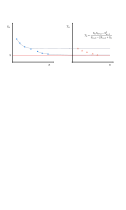
\includegraphics{figures/aitken}
  \caption{Geometrical interpretation of Aitken's \(\Delta^2\) method.}
  \label{fig:aitken}
\end{figure}

One can also show that if \((S_n)\) goes to its limit \(S\) at a rate strictly greater than \(1\)\footnote{$(S_{n})$, ${n \in \mathbb{N}}$ converges linearly to $S$ if there exists a number $\mu \in(0,1)$ such that \(\lim_{n \rightarrow \infty} \frac{\left|S_{n+1}-S\right|}{\left|S_{n}-S\right|}=\mu\).}, \((T_n)\) does not have a better rate of convergence.

In practice, the sequence produced by Aitken's \(\Delta^2\) method tends to converge faster to the limit than \((S_n)\) does.
Very often, it is much cheaper to calculate \((T_n)\), which involves only the calculation of differences, one multiplication, and one division, than to calculate many more terms of the sequence \((S_n)\).
Care must be taken, however, to avoid introducing errors due to insufficient precision when calculating the differences in the numerator and denominator of the expression.

There is, however, no universal sequence accelerator capable of accelerating all sequences.
It is also the case that nonlinear transformations can even fail to converge or converge to a value other than the limit of the original sequence \citep{brezinski_extrapolation_2013}.

According to \cite{brezinski_extrapolation_2013}, there is a very strong connection between sequence transformations and fixed point methods for solving \(x= g( x)\), \(g\colon \mathbb R\to \mathbb R\).
The most well-known example of this connection is that between Aitken's \(\Delta^{2}\) process and Steffensen's method.
\begin{equation}
T_{n}=S_{n}-\frac{\left(S_{n+1}-S_{n}\right)^{2}}{S_{n+2}-2 S_{n+1}+S_{n}}, \quad n=0,1, \ldots \quad\text{for Aitken's process}
\end{equation}
and
\begin{equation}
x_{n+1}=x_{n}-\frac{\left(g\left(x_{n}\right)-x_{n}\right)^{2}}{g\left(g\left(x_{n}\right)\right)-2 g\left(x_{n}\right)+x_{n}},\quad n=0,1, \ldots \quad\text{for Steffensen's method.}
\end{equation}

Turning to vector sequences and systems of nonlinear equations, let \(F:(\mathbf w^{k}) \to(\mathbf y^{k})\) be a vector extrapolation method defined by
\begin{equation}
\mathbf y^k = F\left(\mathbf w^{k}, \ldots, \mathbf w^{k+m}\right), \quad n=0,1, \ldots
\end{equation}
For solving the fixed point problem \(\mathbf x=\pazocal S(\mathbf x)\) one can associate to it the iterative method
\begin{equation}
\mathbf x^{k+1}=F\left(\mathbf x^{k}, \pazocal S(\mathbf x^{k}), \ldots, \pazocal S^{m}(\mathbf x^{k})\right), \quad n=0,1, \ldots
\end{equation}
where \(\pazocal S^{m+1}(\mathbf x)=\pazocal S \circ \pazocal S^{m}(\mathbf x)\) and \(\pazocal S^{0}(\mathbf x)=\mathbf x\).
This approach is called full cycling or simply cycling.
Conversely to any fixed point iteration of this form, one can associate a sequence transformation of the previous form.
See Box~\ref{box:vector_extrapolation_cycling} for the general algorithm, excluding the extrapolation method.

\begin{framedbox}[htbp]
  \caption{Timestep \(n\) of vector extrapolation with cycling.}
  \label{box:vector_extrapolation_cycling}
  \begin{center}
    \begin{minipage}{0.9\textwidth}
    \begin{enumerate}[(i)]
    \item Choose integers \(n\geq 0\) and \(k\leq 1\) and an initial vector \(\mathbf x^k =\mathbf x^*_0\).
    \item Compute \(\mathbf x^*_1\), \(\mathbf x^*_2\), \dots, \(\mathbf x^*_{n+k+1}\) via \(\mathbf x^*_{m+1} = \pazocal S(\mathbf x^*_m)\).
    \item Apply any of the four extrapolation methods, namely, MPE, RRE, MMPE, and SVD-MPE, to \(\mathbf x^*_n\), \(\mathbf x^*_{n+1}\), \dots, \(\mathbf x^*_{n+k+1}\), obtaining \(\mathbf s_{k,n}\).
    \item If \(\mathbf s_{n,k}\) satisfies the accuracy test, stop.\\
    Otherwise, set \(\mathbf x^*_0=\mathbf s_{n,k}\) and go to Step (ii).
    \end{enumerate}
    \end{minipage}
  \end{center}
\end{framedbox}

There is a variety of vector extrapolation methods, where the major two categories are polynomial methods and methods based on the \(\epsilon\)-algorithm \citep{brezinski_extrapolation_2013, sidi_vector_2017}.
In this presentation, only the first category is considered since the second requires a relatively large number of function evaluations per iteration, making it unsuitable for the present use-case \citep{sidi_vector_2017}.

\cite{sidi_vector_2017} presents four different polynomial extrapolation methods.
They all attempt to exprress the limit of the vector sequence as a linear combination of the \(p\) previous iterates, as follows
\begin{equation}
\mathbf s \approx \mathbf{s}_{k, m}=\sum_{j=0}^{m} \gamma_{j} \mathbf w^{k+j},
\end{equation}
where \(\mathbf s\) is the limit of the vector sequence.
The methods to be presented next appear naturally when considering the vector sequence generated by
\begin{equation}
  \mathbf w^{k+1} = \mathbf{T}\mathbf w^k +\mathbf d,
\end{equation}
where \(\mathbf I - \mathbf T\) is non-singular.
It is tighly connected to the solution of linear systems of equations.
Considering the minimal polynomial of \(\mathbf T\) with respect to \(\Delta \mathbf w^{k} = \mathbf w^{k+1} -\mathbf w^k\) and \(\boldsymbol \epsilon^k = \mathbf w^k - \mathbf s\)\footnote{A polynomial \(P(\lambda)\) is said to be minimal with respect to a vector \(\mathbf a\), if \(P(\mathbf T) \mathbf a = 0\) and it of least degree.}, \(P(\lambda)\),
\begin{equation}
  P(\lambda ) = \sum_{j=0}^i c_j \lambda^j, \quad c_i=1,
\end{equation}
where \(i\) is the degree of the polynomial, the limit of the sequence can be found exactly as
\begin{equation}
  \mathbf s = \frac{ \sum_{j=0}^i c_j \mathbf w^{k+j}}{ \sum_{j=0}^i c_j}.
\end{equation}

This can be derived considering the definition of \(P(\lambda)\), \(P(\mathbf T) \boldsymbol \epsilon^k=0\).
Therefore,
\begin{equation}
\mathbf 0=P(\mathbf T) \boldsymbol \epsilon^{k}=\sum_{j=0}^{i} c_{j} \mathbf T^{j}  \boldsymbol\epsilon^{j}=\sum_{j=0}^{i} c_{j} \boldsymbol \epsilon^{k+j}.
\end{equation}
and so
\begin{equation}
0=\sum_{i=0}^{k} c_{i} \boldsymbol{\epsilon}_{n+i}=\sum_{i=0}^{k} c_{i} \boldsymbol{x}_{n+i}-\left(\sum_{i=0}^{k} c_{i}\right) \mathbf{s}.
\end{equation}
Solving this for \(\mathbf s\), one obtains the desired result, provided \(\sum_{j=0}^{i} c_{j} \neq 0\).

The coefficients of \(P(\lambda)\) can be computed considering
\begin{equation}
\mathscr W^{i-1} \mathbf c^{\prime}=-\Delta \mathbf w_{k+i}, \quad \mathbf c^{\prime}=\left[c_{0}, c_{1}, \ldots, c_{i-1}\right]^{T},
\end{equation}
where \(\mathscr W^i = [\Delta \mathbf w^k, \dots, \Delta \mathbf w^{k+i}]\), since from the defintion of \(P(\lambda)\), one has
\begin{equation}
  \mathbf 0 = P(\mathbf T) \Delta \mathbf w^k = \sum_{j=0}^i c_i \mathbf T^j \Delta \mathbf w^k = \sum_{j=0}^i c_i \Delta \mathbf w^{k+j}.
\end{equation}

The degree of \(P(\lambda)\) can be as large as the dimension of \(\mathbf w\).
Hence, to be practical, the minimal polynomial extrapolation (MPE), the reduced rank extrapolation (RRE), the modified minimal extrapolation (MMPE), and the single-value decomposition, minimal polynomial extrapolation (SVD-MPE) all choose a polynomial of a lesser degree.
The approximations corresponding to each extrapolation method are presented in what follows.

\paragraph{MPE}

Solve the overdetermined linear system \(\mathscr W^{m-1} \mathbf c^{\prime}=-\Delta \mathbf w_{k+m}\) in the least-squares sense for \(\mathbf c^{\prime}=\left[c_{0}, c_{1}, \ldots, c_{m-1}\right]^{T}\).
This amounts to solving the optimization problem
\begin{equation}
\min _{c_{0}, c_{1}, \ldots, c_{p-1}}\left\|\sum_{j=0}^{m-1} c_{j} \Delta \mathbf w^ {k+j}+\Delta \mathbf w^{k+m}\right\|_2
\end{equation}
which can also be expressed as
\begin{equation}
  \min _{\mathbf c^{\prime}}\left\|\mathscr W^{m-1} \mathbf c^{\prime}+\mathbf w^{k+m}\right\|_2, \quad \mathbf c^{\prime}=\left[c_{0}, c_{1}, \ldots, c_{m-1}\right]^{T} .
\end{equation}
With \(c_{0}, c_{1}, \ldots, c_{k-1}\) available, set \(c_{m}=1\) and compute \(\gamma_{q}=c_{q} / \sum_{j=0}^{m} c_{j}, q=0,1, \ldots, m\), provided \(\sum_{j=0}^{m} c_{j} \neq 0\).

\paragraph{RRE}

Solve the overdetermined linear system \(\mathscr W^{m} \boldsymbol\gamma=0\) in the least-squares sense, subject to the constraint \(\sum_{j=0}^{m} \gamma_{j}=1\).
This amounts to solving the optimization problem
\begin{equation}
\min _{\gamma_{0}, \gamma_{1}, \ldots, \gamma_{m}}\left\|\sum_{j=0}^{m} \gamma_{j} \Delta\mathbf w^{k+j}\right\| \text { subject to } \sum_{j=0}^{m} \gamma_{j}=1
\end{equation}
which can also be expressed as
\begin{equation}
\min _{\boldsymbol\gamma}\left\|\mathscr W^{m} \boldsymbol\gamma\right\|_2 \quad \text { subject to } \sum_{j=0}^{m} \gamma_{j}=1 ; \quad \boldsymbol\gamma=\left[\gamma_{0}, \gamma_{1}, \ldots, \gamma_{m}\right]^{T} .
\end{equation}

\paragraph{MMPE}

Consider a set of \(m\) linearly independent vectors \(\mathbf q_j\), \(j=1, \dots, m\).
Solve the linear system
\begin{equation}
  \left(\mathbf q^{j}, \mathscr W^{m-1} \mathbf c^{\prime}\right)=-\left(\mathbf q^{j}, \Delta \mathbf w^{k+m}\right), \quad j=1, \ldots, m,
\end{equation}
which can also be expressed as
\begin{equation}
  \sum_{j=0}^{m-1}\left(\mathbf q_{j}, \Delta \mathbf w^{k+j}\right) \mathbf c_{j}=-\left(\mathbf q^{j}, \Delta \mathbf w^{k+p}\right), \quad j=1, \ldots, m.
\end{equation}
This is, in fact, a system of \(m\) linear equations for the \(m\) unknowns \(c_{0}, c_{1}, \ldots, c_{m-1}\).
With \(c_{0}, c_{1}, \ldots, c_{m-1}\) available, set \(c_{m}=1\) and compute \(\gamma_{q}=c_{q} / \sum_{j=0}^{m} c_{j}, i=0,1, \ldots, m\), provided \(\sum_{j=0}^{m} c_{j} \neq 0\).

\paragraph{SVD-MPE}

Solve the standard \(l_{2}\) constrained minimization problem
\begin{equation}
  \min_{\mathbf c}\left\|\mathscr W^{m} \mathbf c\right\|_{2} \quad \text { subject to }\|\mathbf c\|_{2}=1, \quad \mathbf c=\left[c_{0}, c_{1}, \ldots, c_{m}\right]^{T} .
\end{equation}
The solution \(\mathbf c\) is the right singular vector corresponding to the smallest singular value \(\sigma_{\min }\) of \(\mathscr W^{m}\), i.e., \({\mathscr W^{m}}^{*} \mathscr W^{m} \mathbf c=\sigma_{\min }^{2} \mathbf c\), \(\|\mathbf c\|_{2}=1\).
It is assumed that \(\sigma_{\min }\) is simple so that \(\mathbf c\) is unique up to a multiplicative constant \(\phi\), \(|\phi|=1\).

With \(c_{0}, c_{1}, \ldots, c_{m}\) available, compute \(\gamma_{q}=c_{q} / \sum_{j=0}^{m} c_{j}, q=0,1, \ldots, m\), provided \(\sum_{j=0}^{m} c_{j} \neq 0\).
The assumption that \(\sigma_{\min }\) is simple guarantees the uniqueness of the \(\gamma_{i}\).

When \(m=1\), MPE, RRE, MMPE, and SVD-MPE can be regarded as generalizations of the Aitken \(\Delta^2\)-process to the vector case.
Thus, when applied to the solution of a system of nonlinear equations using cycling
\begin{equation}
\mathbf{s}_{k, 1}=\begin{cases}
\mathbf x^{k}-\displaystyle\frac{\left(\Delta \mathbf x^{k}, \Delta \mathbf x^{k}\right)}{\left(\Delta \mathbf x^{k}, \Delta^{2} \mathbf x^{k}\right)} \Delta \mathbf x^{k} & \text { for MPE, } \\[10pt]
\mathbf x^{k}-\displaystyle\frac{\left(\Delta^{2} \mathbf x^{k}, \Delta\mathbf  x^{k}\right)}{\left(\Delta^{2} \mathbf x^{k}, \Delta^{2} \mathbf x^{k}\right)} \Delta \mathbf x^{k} & \text { for RRE, } \\[10pt]
\mathbf x^{k}-\displaystyle\frac{\left(\mathbf  q_{1}, \Delta \mathbf x^{k}\right)}{\left(\mathbf  q_{1}, \Delta^{2} \mathbf  x^{k}\right)} \Delta \mathbf x^{k} & \text { for MMPE, } \\[10pt]
\mathbf x^{k}-\displaystyle\frac{\left(\mathbf g_{0}, \Delta\mathbf x^{k}\right)}{\left( \mathbf g_{0}, \Delta^{2} \mathbf x^{k}\right)} \Delta \mathbf  x^{k} & \text { for SVD-MPE. }
\end{cases}
\end{equation}

\cite{sidi_vector_2017} also suggest cycling with frozen \(\gamma_i\), where after some iterations the \(\gamma_i\) are frozen and reused henceforth.
A parallel version of the full cycling procedure is also described.

\paragraph{Connection to Krylov subspace methods}

According to \cite{sidi_vector_2017}, the so-called Krylov subspace methods are closely related to the vector extrapolation methods presented above.
When the latter is applied to vector sequences obtained using fixed-point iterative methods to nonsingular linear systems of equations, they are mathematically equivalent.
More precisely, the MPE and the RRE methods are mathematically equivalent to the methods of Arnoldi and generalized minimal residual (GMR).

However, Krylov subspace methods and extrapolation methods differ in their algorithmic aspects entirely:
The only input of the former is a procedure that performs the matrix-vector multiplication without explicitly knowing the matrix coefficient matrix.
The latter takes as their only input a vector sequence that results from a fixed-point iterative scheme without knowing the matrix coefficient.

In \cite{michler_interface_2005}, a Krylov-subspace method is proposed in the context of FSI.
However, as pointed out by \cite{kuttler_vector_2009}, the correct term for this approach should be instead a "Krylov-based vector extrapolation" method.
The method proposed can be obtained by applying the RRE to the sequence of residuals computed as
\(\Delta \mathbf r^*_i = \mathbf x^*_i - \mathbf x^k\), where the subscript \(i\) concerns the internal loop of the vector extrapolation method, and whose limit is \(\mathbf 0\).
\cite{kuttler_vector_2009} argues that these residual differences have unfavorable numerical properties and should be avoided.


% \Floatbarrier

\section{Multipoint iteration functions with memory}

Multipoint iteration functions are rarer and are not thoroughly investigated in this exposition.
One can mention the Eirola-Nevanlinna family of methods \citep{fang_two_2009} and Netwon-Krylov method that reuses the Krylov subspace from previous iterations \citep{sidi_vector_2017}.

\section{Summary}

The overview provided in this chapter centered on implicit techniques for partitioned multi-physics coupled applications.
The problem can be slightly reformulated as a system of nonlinear equations, where the residual represents the difference between the input and output after the fixed-point procedure has been applied.
This allows the problem to be solved using a variety of methods described in the literature to tackle system of nonlinear equations.
The key issues in the current application are the memory requirements of the numerical technique due to a potential high number of unknowns and the number of residual evaluations, as each assessment necessitates a significant computational effort.
Table~\ref{tab:mem_nr_func_eval_obs} provides information on the memory requirements, the number of function evaluations per nonlinear iteration, and some pertinent observations for each technique under consideration.

Except for the MMPE and SVD-MPE approaches, the computational performance of all the methods discussed in the present chapter are analyzed in the next chapter (Chapter~\ref{ch:val_acc_techniques}).
As seen in Table~\ref{tab:form_nonlin_methods}, where the update formulae for the methods are compiled, their implementation is made simpler by the similarities in the update formula for the value of the unknown variable at each nonlinear iteration.


\begin{landscape}
\begin{table}[htbp]
  \caption{Summary of the comparison between method for the solution methods of non-linear systems of equations. \(n\) here denotes the number of unknowns and \(m\) denotes depending on the context the number of previous iterates considered, the number of fixed point evaluations or the size of the Krylov subspace.}
\label{tab:mem_nr_func_eval_obs}
  % \setlength{\tabcolsep}{1pt}
  \centering
    \begin{tabular}{l cc p{10.5cm}}
    Method & \makecell[c]{Memory\\requirements} & \makecell[c]{Nr function\\evaluations\\per iteration} & Observations\\
    \hline  \hline
    \multirow{3}{*}{\vphantom{\Big|}Fixed-point iteration} & \multirow{3}{*}{2 \((n\times 1)\) vectors} & \multirow{3}{*}{1} & \textbullet Often diverges.\\
    & & &\textbullet Simplest method.\\
    & & &\textbullet Memory efficient.\\
    \hline
    \multirow{3}{*}{Underrelaxation} & \multirow{3}{*}{2 \((n\times 1)\) vectors} & \multirow{3}{*}{1} & \textbullet Simple.\\
    & & &\textbullet Improved stability over fixed-point.\\
    & & &\textbullet Need to manually choose a relaxation parameter.\\
    \hline
    \multirow{3}{*}{Aitken relaxation} & \multirow{3}{*}{3 \((n\times 1)\) vectors} & \multirow{3}{*}{1} & \textbullet Very popular in FSI.\\
    & & & \textbullet Dynamic relaxation.\\
    & & & \textbullet Improved stability over fixed-point.\\
    \hline
    \multirow{3}{*}{\makecell[l]{Broyden-like family\\\citep{fang_two_2009}}} & \multirow{3}{*}{\makecell[c]{2 \((n\times 1)\) vectors\\2 \((n\times (m-1))\) matrices}} & \multirow{3}{*}{1} & \textbullet \(\pazocal O(nm^2)\) computation complexity (\(QR\) decomposition). \\
    & & & \textbullet Low number of function evaluations\\
    & & & \textbullet Superlinear convergence when \(m=1\).\\
    \hline
    \multirow{3}{*}{\makecell[l]{Broyden's method\\\citep{kelley_solving_2003}}} & \multirow{3}{*}{\makecell[c]{Up to\\ \((m+2) (n\times 1)\) matrices}} & \multirow{3}{*}{1} & \textbullet \(\pazocal O(n)\) computation complexity.\\
    & & & \textbullet Low storage.\\
    & & & \textbullet Superlinear convergence.\\
    \hline
    \multirow{3}{*}{Newton-Krylov} & \multirow{3}{*}{\makecell[c]{Up to\\\((m+1)\) \((n\times 1)\) vectors}} & \multirow{3}{*}{\(m+1^*\)} & \textbullet Large number of iterations possible.\\
    & & & \textbullet Popular for the solution of systems of nonlinear equations.\\
    & & & \textbullet Quadratic convergence under appropriate conditions.\\
    \hline
    \multirow{2}{*}{\makecell[l]{Vector extrapolation\\ in cycling mode}} & \multirow{2}{*}{\((m+2)\) \((n\times 1)\) vectors} & \multirow{2}{*}{\(m+1\)} & \textbullet Large number of function evaluations.\\
    & & & \textbullet \(\pazocal O(nm^2)\) computational complexity (\(QR\) decomposition).\\
  \hline\hline
  \multicolumn{4}{l}{\vphantom{\Huge |}\parbox{\textwidth}{\footnotesize{  \(^*\) The number of function evaluations in the Newton-Krylov methods will depend on how many iterations it will take for the inner loop to converge. There is a function evaluation per iteration of the inner loop.}}}
  \end{tabular}
\end{table}
\end{landscape}



\begin{table}[htbp]
  \caption{Summary of the update formulas for the solution methods of non-linear systems of equations.}
\label{tab:form_nonlin_methods}
  % \setlength{\tabcolsep}{1pt}
  \centering
    \begin{tabular}{l c}
    Method & Update formula\\
    \hline\hline
    \vphantom{\Huge |}Fixed-point &  \makecell[l]{\(\mathbf x^{k+1} = \mathbf x^k -  \pazocal R^k\)}\\
    \hline
    Underrelaxation & \makecell[l]{\vphantom{\Huge |}\(\mathbf x^{k+1} = \mathbf x^k - \omega\pazocal R^k\),\\\(0<\omega<1\).}\\
    \hline
    Aitken relaxation & \makecell[l]{\vphantom{\Huge |}\(\mathbf x^{k+1} = \mathbf x^k - \omega^{(k)}\pazocal R^k\),\\    \(\omega^{(k)}=-\omega^{(k-1)} \displaystyle\frac{\left(\mathbf{r}^{(k)}-\mathbf{r}^{(k-1)}\right)^{\mathrm{T}} \mathbf{r}^{(k-1)}}{\left(\mathbf{r}^{(k)}-\mathbf{r}^{(k-1)}\right)^{2}}.\)
    }\\
    \hline
    Broyden's family & \makecell[l]{\vphantom{\Huge |} \(\mathbf x^{k+1} = \mathbf x^{k}- \left(G_\pazocal R^{k-m} +\left(\mathscr{X}^{k}-G_\pazocal R^{k-m} \mathscr{R}^{k}\right){\mathbf V^k}^T\right) \pazocal R^k,\)\\
    \({\mathbf V^k}^T = {\mathbf M^k}^{-1}{\mathbf N^k}^T\),\\
    Type I:  \({M^k} = {\mathscr X^k}^T G_\pazocal R^k \mathscr R^k,\quad {N^k}^T = {\mathscr X^k}^T G_\pazocal R^k,\)\\
    Type II: \({M^k} = {\mathscr R^k}^T \mathscr R^k,\quad {N^k}^T = {\mathscr R^k}^T\)\\
    {\small \(\mathbf V^k\) is usually computed using \(QR\)-decomposition.}
    }\\
    \hline
    Anderson's family & \makecell[l]{\vphantom{\Huge |} \(\mathbf x^{k+1} = \mathbf x^{k} -\left(-\beta \mathbf I+\left(\mathscr{X}^{k}+\beta \mathscr{R}^{k}\right){\mathbf V^k}^T\right) \pazocal R^k,\)\\
    \({\mathbf V^k}^T = {\mathbf M^k}^{-1}{\mathbf N^k}^T\),\\
    Type I:  \({M^k} = {\mathscr X^k}^T \mathscr R^k,\quad {N^k}^T = {\mathscr X^k}^T ,\)\\
    Type II: \({M^k} = {\mathscr R^k}^T \mathscr R^k,\quad {N^k}^T = {\mathscr R^k}^T\)\\
    {\small \(\mathbf V^k\) is usually computed using \(QR\)-decomposition.}
    }\\
    \hline
    Newton-Krylov & \makecell[l]{\vphantom{\Huge |} \(\mathbf x^{k+1} = \mathbf x^{k} +\Delta \mathbf x^k\)\\
    \(J_\pazocal R(\mathbf x^k)\Delta x^k = -\pazocal R^k\) solved using a Krylov method\\
    to accuracy \(  \|J_\pazocal R(\mathbf x^k) \Delta x^*_m+ \pazocal R(\mathbf x^k)\| \leq \eta\|\pazocal R(\mathbf x^k)\|\)}
    \\
    \hline
    \makecell[l]{Vector extrapolation\\ in cycling mode} & \makecell[l]{\vphantom{\Huge |}
    \(\mathbf x^{k+1} = \sum_{j=0}^m \gamma_j \pazocal S^{i+j}(\mathbf x^k)\),\\
    \(\gamma_q = c_q/\sum_j c_j,\quad q=0,1,\dots,m,\)\\
    \textbf{MPE}: \(\mathbf c ' = [c_0,c_1,\dots,c_{m-1}]^T = \arg \min_{\bar{\mathbf c}} \left\|\mathscr S^{m-1} \bar{\mathbf c}^\prime + \pazocal S^{i+m}(\mathbf x^k)\right\|_2\),\\
    \(c_m=1\),\\
    \textbf{RRE}: \(\boldsymbol{\gamma} = [\gamma_0,\gamma_1,\dots,\gamma_{m}]^T = \arg \min_{\bar{\boldsymbol{ \gamma}}} \left\|\mathscr S^{m} \hat{\boldsymbol{\gamma}}\right\|_2\),\\
    Subject to \(\sum_{j=0}^m \gamma_j =1\).\\
    \textbf{MMPE}: \(\left(\mathbf q^{j}, \mathscr S^{m-1} \mathbf c^{\prime}\right)=-\left(\mathbf q^{j}, \pazocal S^{i+m}(\mathbf x^k)\right), \quad j=1, \ldots, m,\)\\
    for a set of \(m\) linearly independent vectors \(\mathbf q_j\), \(j=1, \dots, m\).\\
    \(\mathbf c ' = [c_0,c_1,\dots,c_{m-1}]^T.\)\\
    \textbf{SVD-MPE}: \(\mathbf c = \arg\min_{\bar{\mathbf c}}\left\|\mathscr S^{m} \bar{\mathbf c}\right\|_{2} \quad \text { subject to }\|\bar{\mathbf c}\|_{2}=1,\)\\
    \(\mathbf c=\left[c_{0}, c_{1}, \ldots, c_{m}\right]^{T}\).
    }\\
  \hline\hline
  \end{tabular}
\end{table}

\FloatBarrier

\newpage\null\thispagestyle{blank}\newpage
